\documentclass[a4,abstract=on]{scrartcl}

\usepackage[utf8]{inputenc}
\usepackage[T1]{fontenc}
\usepackage{placeins}
\usepackage{amsthm }
\usepackage{graphicx}
\usepackage[hypcap]{caption}
\usepackage{algorithm}
\usepackage[noend]{algpseudocode}
\usepackage[hidelinks]{hyperref}
\usepackage[nochapters]{classicthesis} % nochapters, wenn du section als oberste ebene nimmst
\usepackage{array}
\usepackage{mdframed}
\usepackage{datatool}
\usepackage{dataplot}

\DTLsetseparator{;}
\PassOptionsToPackage{big}{titlesec}

\floatname{algorithm}{Algorithmus}
% Mathe
\usepackage{amsmath}
\usepackage{amssymb}


% Verlinkungen
\usepackage[ngerman]{varioref} % Siehe http://en.wikibooks.org/wiki/LaTeX/Labels_and_Cross-referencing#The_varioref_package
%\usepackage[hidelinks]{hyperref}

% Spracheinstellungen sowie Umlaute etc.
\usepackage[ngerman]{babel}
\usepackage{ngerman}

% Bilder
\usepackage{graphicx}

% Tabellen-Abstand
\renewcommand{\arraystretch}{1.5}

% Quellcode
\usepackage{listings}
\lstset{%
	breaklines=true,
	frame=single,
	keepspaces=true,
	numbers=left,
	numbersep=5pt,
	tabsize=2
}

% Literatur
\usepackage{bibgerm}
\usepackage{natbib}

% Lässt sections immer auf der ungeraden (rechten) Seite anfangen.
    \newcommand*\stdsection{}
    \let\stdsection\section
    \renewcommand*\section{%
    \clearpage\ifodd\value{page}\else\mbox{}\clearpage\fi
    \stdsection}

% neuer Typ von Tabellenspalte (so wie c, l, etc.). Ist zentriert mit fester Breite.
\newcolumntype{C}[1]{>{\centering\let\newline\\\arraybackslash\hspace{0pt}}m{#1}}

% \usepackage{setspace}
% \onehalfspacing
\title{Untersuchung verschiedener Kodierungen von speziellen Cardinality Constraints für SAT}
\date{~}

\begin{document}



	\maketitle
\thispagestyle{empty}
\begin{center}
\begin{Large}
Bachelorarbeit\\Universität Bremen\\Fachbereich $3$\\
~\\~\\
\textbf{Jil Tietjen}\\<jiltietj@informatik.uni-bremen.de>\\
~\\~\\
Erstgutachter: Prof. Dr. Rolf Drechsler\\
Zweitgutachter: Prof. Dr. Rüdiger Ehlers\\~\\
\mbox{Betreuung: Prof. Dr. Rolf Drechsler \&~Oliver Keszöcze}\\~\\~\\~\\~\\~\\~\\~\\
Bremen, $09$. Juni $2016$
\end{Large}
\end{center}
		
	\newpage
~\\
\textbf{Urheberrechtliche Erklärung}\\
Erklärung gem. § $10$ ($10$) Allgemeiner Teil der BPO vom $27$.$10$.$2010$
Hiermit versichere ich, dass ich meine Bachelorarbeit ohne fremde Hilfe angefertigt habe, und dass ich keine anderen als die von mir angegebenen Quellen und Hilfsmittel benutzt habe.\\
Alle Stellen, die wörtlich oder sinngemäß aus Veröffentlichungen entnommen sind, habe ich unter Angabe der Quellen als solche kenntlich gemacht.\\
Die Bachelorarbeit darf nach Abgabe nicht mehr verändert werden.\\
~\\~\\~\\
Bremen, den $09$.$06$.$2016$\\
~\\~\\~\\
Jil Tietjen
~\\~\\~\\~\\~\\~\\
Ich bin damit einverstanden, dass meine Abschlussarbeit im Universitätsarchiv für wissenschaftliche Zwecke von Dritten eingesehen werden darf.\\
~\\~\\~\\
Bremen, den $09$.$06$.$2016$\\
~\\~\\~\\
Jil Tietjen
\clearpage

	\tableofcontents
	\clearpage

\section{Einleitung}
Viele praktische Probleme in der Informatik, zum Beispiel im Bereich der Bio-Chips, können durch das Umwandeln in bekannte abstrakte Probleme gelöst werden.\\
In den letzten Jahren wurde das Interesse geweckt, diese Probleme mit Cardinality Constraints und SAT-Solvern zu behandeln. In der Vergangenheit wurden diese Kodierungen nicht oder nur begrenzt für praktische Probleme getestet. Die Cardinality Constraints können dafür nicht einfach verwendet werden. Damit sie durch den SAT-Solver verarbeitet werden können, müssen sie in die Sprache der Aussagenlogik, oder besser noch in die konjunktive Normalform kodiert werden. Es gibt jedoch noch keine allgemeine Definition über die beste Kodierung für die Cardinality Constraints. Es lässt sich nur feststellen, dass es von Vorteil ist, wenn die Formel im Hinblick auf die Anzahl der Variablen und Klauseln so klein wie möglich gehalten wird \cite[][]{einleitung}.\\
In dieser Arbeit werden verschiedene Kodierungen für die Cardinality Constraints anhand von Benchmark-Problemen untersucht. Es werden das n-Damen-Problem und Digital Tomography als Testprobleme genutzt. Des Weiteren gibt es zufällig generierte Testfälle, die Cardinality Constraints unterschiedlicher Größe untersuchen. \\
Die Kodierungen, die binär oder unär sind, basieren auf unterschiedlichen Methoden. Dazu gehören binäre Bäume, Schaltkreise (Addierer), Binary Decision Diagrams oder Sorting Networks mit verschiedenen Sortieralgorithmen. \\
Außerdem wurde in dieser Arbeit eine eigene Kodierung, basierend auf Sorting Networks, entwickelt. Hier soll vor allem hinsichtlich des Speicherbedarfs eine Optimierung gegenüber anderen etablierten Verfahren erreicht werden. Dies geschieht durch das Entfernen nicht benötigter Comparators im Sorting Network. \\
Ziel dieser Arbeit ist es, die untersuchten Kodierungen für diese praktischen Probleme zu vergleichen. Hierbei wird der Speicher- und Zeitbedarf für das Lösen der Probleme gemessen. \\
\newline
Der Rest dieser Arbeit teilt sich in folgende Abschnitte: in Abschnitt $2$ werden die notwendigen Grundlagen für diese Arbeit vermittelt. Dazu gehören das SAT-Problem mit dem SAT-Solver und den Cardinality Constraints sowie die Tseitin-Transformation und Sorting Networks, die bei mehreren Kodierungen eingesetzt werden.\\
Der nächste Abschnitt erläutert die unterschiedlichen Kodierungen mit einigen Beispielen, die das Vorgehen der Algorithmen besser verdeutlichen. In diesem Abschnitt wird als Letztes die eigene Kodierung vorgestellt.\\
In Abschnitt $4$ werden die Ergebnisse der Evaluation dargelegt. \\
Das letzte Kapitel fasst alle Kernelemente der Arbeit zusammen und gibt einen Ausblick auf mögliche weitere Themen für Anschlussarbeiten.


\section{Grundlagen}
%n in den Grundlagen erklären
In diesem Kapitel werden alle notwendigen Grundlagen für das Verständnis dieser Bachelorarbeit dargelegt. Es dient als Einführung in das Thema, so dass alle benutzten Kodierungen nachvollzogen werden können.
\subsection{SAT-Problem}
Das Satisfiability Problem (kurz: SAT) ist das Erfüllbarkeitsproblem der Aussagenlogik \cite[vgl.][]{sat-problem}. Es ist NP-vollständig und lässt sich daher vermutlich nicht in polynomieller Zeit lösen. Die Eingabe ist eine aussagenlogische Formel F, für die herausgefunden werden soll, ob sie erfüllbar ist. Es wird also eine erfüllende Belegung der Variablen mit true oder false gesucht.\\
Eine Formel ist ein wohlgeformter Ausdruck, für den folgende Regeln gelten:

\begin{mdframed} [linecolor=black,linewidth=2pt]
Eine Aussagenvariable oder Konstante ist eine Formel.\\
Ist $F$ eine Formel, dann ist auch  $\neg F$  eine Formel.\\
Sind $F$ und  $Q$  Formeln, dann sind
$F \wedge Q  \text{ und }  F \vee Q \text{ auch Formeln.}$\\
$F(P\wedge Q) = \begin{cases}1 \text{, gdw. } F(P) = 1 \text{ und } F(Q)=1\\ 0 \text{ sonst}\end{cases}$\\
$F(P\vee Q) = \begin{cases}0 \text{, gdw. } F(P) = 0 \text{ und } F(Q)=0\\ 1 \text{ sonst}\end{cases}$\\
$F(\neg P) = \begin{cases}0 \text{, gdw. } F(P) = 1 \\ 1 \text{, gdw } F(P) = 0\end{cases}$
\end{mdframed}
\ \\
Die Formel F liegt üblicherweise in Konjunktiver Normalform (KNF) vor. Eine Formel ist in konjunktiver Normalform, wenn sie eine Konjunktion von Klauseln ist. Eine Klausel ist eine Disjunktion von Literalen und ein Literal eine Formel der Form $x$ oder $\neg x$, wobei $x$ eine atomare Variable ist.\\
\begin{align*}
&F = \bigwedge_{i=1, \dots ,n} \bigvee_{j=1,\dots ,m_i}{l_{i,j}}\\
\end{align*}
Eine SAT-Instanz ist zum Beispiel $(\neg a) \wedge (b \vee \neg c \vee d) \wedge (a \vee \neg b)$ mit den Variablen $a,b,c,d$. Für sie gibt es die Lösung: $a = 0,{~} b = 0,{~} c= 0, {~} d = 1$. Es muss eine Belegung gefunden werden, so dass jede Klausel erfüllt ist.
Eine Klausel kann auch als eine endliche Menge von Literalen angesehen werden. Bei einer KNF-Formel wird die Klauselmenge M(F) wie folgt zugeordnet:\\
\begin{itemize}
\item $i$-te Disjunktion $\bigvee_{j=1,\dots ,m_i}{l_{i,j}}$ entspricht Klausel $C_i = \{l_{i1}, \dots, l_{im_i}\}$
\item M(F) = $\{C_1, \dots, C_n\}$
\end{itemize}
\subsubsection{SAT-Solver}
Mit einem SAT-Solver kann für eine Formel in konjunktiver Normalform ermittelt werden, ob sie erfüllbar ist oder nicht. Zur Lösung des Erfüllbarkeitsproblems hat sich der Davis-Putnam-Logemann-Loveland-Algorithmus (kurz: DPLL) durchgesetzt \cite[vgl.][]{dpll}, der ein chronologisches Backtracking umsetzt. Das heißt, dass eine erfüllende Variablenbelegung schrittweise konstruiert und die gegebene Formel dabei vereinfacht wird. Im Folgenden stelle ich den DPLL Algorithmus vor. Die gezeigte Variante ist aus \cite[][]{algoDpll} entnommen und lehnt sich stark an \cite[][]{satisfiability} an.

\FloatBarrier
\begin{algorithm}[h]
\caption{DPLL}
\label{alg:dpll}
\begin{algorithmic}

\State $\text{~~function~}SEARCH(V,\psi,A) $
\State $\text{~~~~}for$ all assignments $v_k=b_k$ implied by $(\psi, A)$ by unit propagation 
\State $\text{~~~~~~}do {~}A:=A\cup\{v_k \rightarrow b_k\}$
\State $\text{~~~~ }end {~} for$
\State $\text{~~~~}if $ some clause in $\psi$ is falsified by $A$ \textit{then}
\State $\text{~~~~~~~~return } \emptyset$
\State $\text{~~~~}end {~} if$
\State $\text{~~~~~~}if {~} |A| = |V| {~} then$
\State $\text{~~~~~~~~return } A$
\State $\text{~~~~~~} end {~} if$
\State $\text{~~~~~~}$Pick a variabe $v$ that is not yet in the domain of $A$
\State $\text{~~~~~~} A' \leftarrow SEARCH(V,\psi,A\cup\{v \rightarrow false\})$
\State $\text{~~~~~~}if$ $A' \neq \emptyset$ \textit{then return} $A'$
\State $\text{~~~~~~}A' \leftarrow SEARCH(V,\psi, A \cup \{v \rightarrow true\})$
\State $\text{~~~~~~}if$ $A' \neq \emptyset$ \textit{then return} $A'$
\State $\text{~~~~return }\emptyset$
\State $\text{~~}$end function
\end{algorithmic}
\end{algorithm}
\FloatBarrier
\ \\
Durch den DPLL-Algorithmus wird versucht Lösungen durch Zuweisungen zu finden. Es ergeben sich dadurch Teillösungen, die sich als erfolgreich oder nicht-erfolgreich erweisen können. \\
Zum Beispiel kann die Formel $(x_1 \vee x_2 \vee x_3) \wedge (\neg x_1 \vee \neg x_4 \vee x_5) \wedge (\neg x_1 \vee x_4)$ mit $x_1=1, x_4=1$ belegt werden. Dann ist die zweite Klausel eine Einheitsklausel, da nur noch $x_5$ übrig bleibt. Damit die Klausel true wird, muss $x_5 = 1$ sein. \\
Wenn eine Klausel durch die aktuelle Zuordnung nicht true ergeben kann, wird durch Backtracking versucht, eine neue Zuordnung zu finden, indem die letzte Entscheidung rückgängig gemacht wird und die Variable davor geändert wird. 
Sobald allen Variablen ein Wert zugewiesen wurde, gibt der Algorithmus \emph{erfüllbar} zurück und ansonsten \emph{unerfüllbar}.\\
Unit Propagation ist ein Verfahren, um aus Einheitsklauseln direkt eine Belegung zu folgern. Eine Klausel ist eine Einheitsklausel, wenn sie genau ein Literal enthält. Um eine Einheitsklausel zu erfüllen, muss die entsprechende Variable mit true beziehnugsweise false belegt werden.\\
Der Algorithmus ist rekursiv und eliminiert in jedem Schritt mindestens eine Variable, wenn möglich durch die Elimination einer Einheitsklausel. Ansonsten wird eine Variable unter Verwendung der Fallunterscheidung mit möglicherweise zwei rekursiven Aufrufen eliminiert.\\
Eine hilfreiche Eigenschaft von SAT-Solvern ist das Klausellernen (CDCL) \cite[][]{cdcl}. Gibt es eine Formel, die auf Grund eines Konfliktes in der Belegung der Variablen nicht erfüllbar ist, wird eine zusätzliche Klausel hinzugefügt. Die neue Klausel schließt die falsche Belegung der entsprechenden Variablen aus, so dass diese Konstellation nicht mehr zu einem Konflikt führen kann.\\
Mit Hilfe der SAT-Solver können NP-vollständige Probleme trotzdem effizient gelöst werden. Durch die hohe Relevanz der Lösung von praktischen Problemen gibt es fast jedes Jahr einen Wettbewerb (\url{http://www.satcompetition.org/}), der neue oder bessere SAT-Solver hervorbringt.

%DPLL
\subsubsection{Cardinality Constraint}
Ein Cardinality Constraint \cite[vgl.][]{sinz} ist eine erweiterte Klausel mit einer Einschränkung der Form 
\begin{align*}
&\sum l_i \leq r, \sum l_i \geq r, oder \sum l_i = r
\end{align*}
\ \\
Für das Cardinality Constraint ist $r$ eine natürliche Zahl und $l_i$ ein Literal. Ein Cardinality Constraint besagt, dass mindestens $r$ der Literale true sein müssen, maximal $r$ der Literale true sein dürfen, beziehungsweise genau $r$ Literale true sein müssen.\\
Für eine Variablenzuordnung $a:V \rightarrow \mathbb{B}$ wird der Wahrheitswert eines Constraints folgendermaßen bestimmt:
\begin{align*}
\hat{a} (\sum(x_1 \dots x_n ) \leq r) = 1 {~~~~} gdw. {~} |\{x_i|\hat{a} (x_i) = 1\}| \leq r \\
\hat{a} (\sum(x_1 \dots x_n ) \geq r) = 1 {~~~~} gdw. {~} |\{x_i|\hat{a} (x_i) = 1\}| \geq r \\
\hat{a} (\sum(x_1 \dots x_n ) = r) = 1 {~~~~} gdw. {~} |\{x_i|\hat{a} (x_i) = 1\}| = r 
\end{align*}
\ \\
Bei diesen Ausdrücken ist $n\geq 0$ und $x_i \in V$ für $1 \leq i \leq n$.\\
Mit Cardinality Constraints können praktische Probleme ausgedrückt werden. Cardinality Constraints können in Konjunktive Normalform übersetzt werden, so dass man SAT-Solver zur Lösung verwenden kann.\\
Im weiteren Verlauf wird nur das <=-Constraint behandelt, da die anderen beiden Constraints damit ausdrückbar sind.
\begin{align*}
&\sum (x_1, \dots, x_n) \geq r \equiv \neg (\sum (x_1, \dots, x_n) \leq (r-1))
\end{align*}
Das Gleiche wird auch für $=$ gemacht.
\begin{align*}
&\sum(x_1, \dots, x_n) = r \equiv \sum(x_1, \dots, x_n) \leq r \wedge \sum(x_1, \dots, x_n) \geq r
\end{align*}


\subsection{Tseitin-Transformation}
Mit Hilfe der Tseitin-Transformation können beliebige aussagenlogische Formeln in konjunktive Normalform gebracht werden \cite [vgl.][]{tseitin}. Dafür werden neue Variablen für jede Subformel hinzugefügt, so dass die resultierende KNF nicht mehr äquivalent, aber immer noch erfüllbarkeitsäquivalent ist. \\
Das bedeutet, dass zwei Formeln $\alpha$ und $\beta$ erfüllbarkeitsäquivalent sind, wenn Folgendes gilt:
$\alpha$ ist erfüllbar gdw. $\beta$ erfüllbar ist.
\ \\
Für jede Subformel $\alpha_1$ von $\alpha$, die kein Atom ist, wird ein neues Atom $t_{\alpha_1}$ hinzugefügt. Die Subformel wird dann nach entsprechenden Regeln der KNF mit $\wedge$ hinzugefügt.\\
\ \\
Dies sind die Regeln der Tseitin Transformation:
\begin{align*}
&\beta \leftrightarrow\neg \beta_1 {~~~~~~~~~~}\rightsquigarrow{~~~~~~~} (\neg t_\beta \vee \neg t_{\beta_1 }) \wedge (t_\beta \vee t_{\beta_1})\\
&\beta \leftrightarrow \beta_1 \wedge \beta_2 {~~~~~~}\rightsquigarrow{~~~~~~} (\neg t_\beta \vee  t_{\beta_1 }) \wedge (\neg t_\beta \vee t_{\beta_2}) \wedge (t_\beta \vee \neg t_{\beta_1} \vee \neg t_{\beta_2})\\
&\beta \leftrightarrow \beta_1 \vee \beta_2 {~~~~~~}\rightsquigarrow{~~~~~~} (t_\beta \vee  \neg t_{\beta_1 }) \wedge (t_\beta \vee \neg t_{\beta_2}) \wedge (\neg t_\beta \vee t_{\beta_1} \vee t_{\beta_2})\\
&\beta \leftrightarrow \beta_1 \rightarrow \beta_2 {~~~~}\rightsquigarrow{~~~~~~} (t_\beta \vee  t_{\beta_1 }) \wedge (t_\beta \vee \neg t_{\beta_2}) \wedge (\neg t_\beta \vee \neg t_{\beta_1} \vee t_{\beta_2})
\end{align*}
\ \\
Beispiel: die folgende Formel $\beta = x_1 \vee (x_2 \wedge (x_3 \rightarrow x_4))$ soll mittels Tseitin-Transformation in eine erfüllbarkeitsäquivalente KNF umgewandelt werden.\\
Es können diese Subformeln gebildet werden:\\
\begin{itemize}
\item $(x_3 \rightarrow x_4)$
\item $x_2 \wedge (x_3 \rightarrow x_4)$
\item $x_1 \vee (x_2 \wedge (x_3 \rightarrow x_4))$
\end{itemize}
\ \\
Für jede Subformel wird eine neue Tseitin-Variable eingeführt.\\
\begin{itemize}
\item $t_1 \leftrightarrow (x_3 \rightarrow x_4)$
\item $t_2 \leftrightarrow x_2 \wedge t_1$
\item $t_3 \leftrightarrow x_1 \vee t_2$
\end{itemize}
\ \\
Im nächsten Schritt wird die KNF aus den Substitutionen gebildet.\\
\begin{align*}
\begin{aligned}
t_1 \leftrightarrow x_3 \rightarrow x_4 &\equiv (t_1 \vee  x_3) \wedge (t_1 \vee \neg x_4) \wedge (\neg t_1 \vee \neg x_3 \vee x_4)\\
t_2 \leftrightarrow x_2 \wedge t_1 &\equiv (\neg t_2 \vee  t_1) \wedge (\neg t_2 \vee x_2) \wedge (t_2 \vee \neg x_2 \vee \neg t_1)\\
t_3 \leftrightarrow x_1 \vee t_2 &\equiv (t_3 \vee  \neg x_1) \wedge (t_3 \vee \neg t_2) \wedge (\neg t_3 \vee x_1 \vee t_2)\\
\end{aligned}
\end{align*}
\ \\
Als Letztes werden alle Substitutionen verbunden.\\
\begin{align*}
& T_\beta \equiv(t_1 \leftrightarrow (x_3 \rightarrow x_4)) \wedge (t_2 \leftrightarrow x_2 \wedge t_1) \wedge (t_3 \leftrightarrow x_1 \vee t_2)
\end{align*}
\ \\
Die vollständige KNF sieht folgendermaßen aus:\\
\begin{align*}
\begin{aligned}
T_\beta \equiv (t_1 \vee  x_3) \wedge (t_1 \vee \neg x_4) \wedge (\neg t_1 \vee \neg x_3 \vee x_4) \wedge (\neg t_2 \vee  t_1) \wedge (\neg t_2 \vee x_2) \wedge \\
(t_2 \vee \neg x_2 \vee \neg t_1) \wedge (t_3 \vee  \neg x_1) \wedge (t_3 \vee \neg t_2) \wedge (\neg t_3 \vee x_1 \vee t_2)
\end{aligned}
\end{align*}

\subsection{BDDs}
Binary Decision Diagrams (BDDs) sind gerichtete Graphen, die für die Darstellung von Booleschen Funktionen benutzt werden \cite[vgl.][Seite 109-110]{bdd}.\\
Ein gerichteter Graph ist ein Paar $G=(V, E)$, wobei $V$ eine Menge von Knoten und $E \subseteq V \times V$  eine Menge von Kanten ist. Ein Knoten wird als Punkt graphisch dargestellt und eine Kante $(v, v')$ durch einen Strich von $v$ nach $v'$. Die Vorgänger eines Knotens $v$ sind die Knoten $v'$, für die es Kanten $(v', v)$ gibt. Die Wurzel ist der Knoten ohne Vorgänger und die Knoten ohne Nachfolger heißen terminale Knoten oder Blätter. Sie werden mit einer $0$ oder einer $1$ markiert. Nicht terminale Knoten $v$ besitzen eine Kante zu einem low- bzw. high- Nachfolger. Sie werden mit Variablen beschriftet. Die Kante $e_1 = (v, low(v))$ nennt man low-Kante und wird mit $0$ markiert. Dies ist in der Regel die linke Kante von einem Knoten. Die high-Kante $e_2 = (v, high(v))$ wird mit einer $1$ markiert und ist die rechte Kante.

\begin{figure}[H]
\centering
\includegraphics[width=4cm]{bdd.png}
\caption{Binary Decision Diagram}
\label{fig:bdd}
\end{figure}
\ \\
Ein BDD repräsentiert in eindeutiger Weise eine Boolesche Funktion. Der Graph aus Abbildung \ref{fig:bdd} kann die Boolesche Funktion $f(x_1,x_2,x_3) = x_1\wedge x_2 \vee x_3$ ausdrücken. Um den Wert einer Funktion für eine feste Belegung abzulesen, folgt man den entsprechenden Kanten im BDD. Zum Beispiel ist $f(1,0,1)=1$.


\subsection{Sorting Networks}
Ein Sorting Network ist ein Network \cite[vgl.][]{sorting}, das aus Comparators besteht. Das Network hat verschiedene Eingangsavariablen, die durch das Anwenden verschiedener Algorithmen mittels der Comparators sortiert werden können. Die Eingangsvariablen können oben an den Ausgängen angeordnet werden, wenn sie mit true belegt sind. Ein einzelner Comparator ist zwischen zwei verschiedenen Leitungen angeordnet. Er hat somit zwei Eingangsvariablen und zwei Ausgangsvariablen, wobei die Ausgangsvariablen so sortiert werden, dass der obere Ausgang den höheren und der untere Ausgang den niedrigeren Wert enthält.

\begin{figure}[H]
\centering
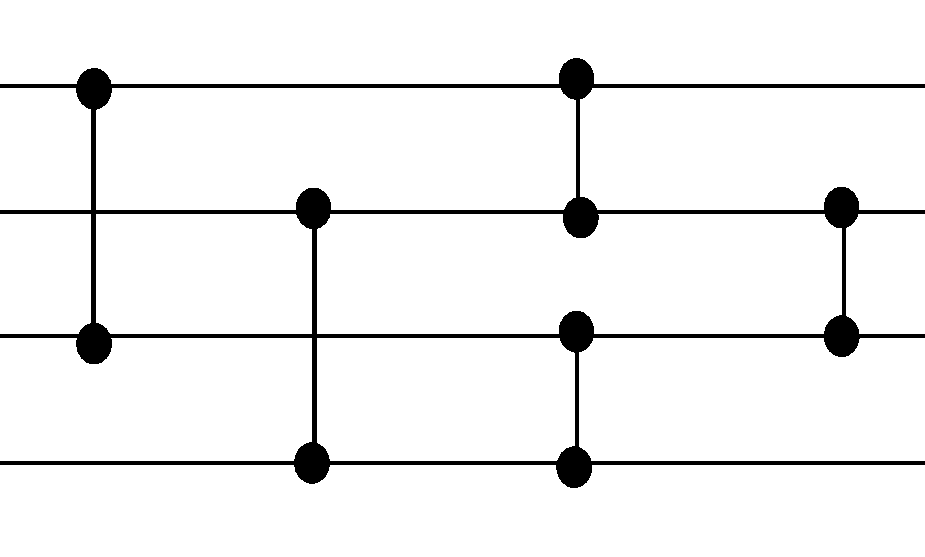
\includegraphics[width=\textwidth]{sorting_network_grundlage1.pdf}
\caption{Beispiel für ein Sorting Network mit Batcher's Merge-Exchange Algorithmus}
\label{fig:network_grundlage}
\end{figure}
\ \\
Die Comparators in einem Sorting Network können nach verschiednen Algorithmen angeordnet werden. Mögliche Algorithmen sind zum Beispiel der Bubble-Sort Algorithmus, der Odd-Even Mergesort Algorithmus oder der Bose-Nelson Algorithmus.

\section{Kodierungen}
In diesem Kapitel werden die unterschiedlichen Kodierungen beschrieben. Das Ziel ist es, dass die Cardinality Constraints über die Menge der Boolschen Variablen in eine Konjunktive Normalform (KNF) gebracht werden. %Innerhalb der KNF gibt es Einschränkungen, die verlangen, dass höchstens $r$ der Booleschen Variablen 1 sein können. Rein in die Grundlagen
Das Cardinalitiy Constraint ist genau dann erfüllt, wenn die aus der Kodierung resultierende Formel erfüllt ist. Ein einzelnes Cardinality Constraint ist immer erfüllbar. Erst eine Kombination mehrerer Cardinality Constraints kann zu einer unerfüllbaren Formel führen.

%Evaluation Alle Kodierungen werden anhand des Damen-Problems und anhand einer Tomography auf ihre Praxistauglichkeit überprüft.

	\subsection{Naiver Ansatz}
Zur Verdeutlichung der Einflüsse der weiteren Kodierungen wird als Erstes der naive Ansatz \cite[][]{sinz} erläutert. Für den Fall $r=1$ wird aus allen möglichen Paaren von Variablen $x_i$ und $x_j$ die Klausel $\neg x_i \vee \neg x_j$ gebildet. Das bedeutet, dass beispielsweise $\sum(x,y,z)\leq1$ zu $(\neg x \vee \neg y) \wedge (\neg x \vee \neg z) \wedge (\neg z \vee \neg y)$ wird.
Für beliebige $r$ gibt es nicht nur Paare von Variablen, sondern $(r+1)$-Tupel.\\
\begin{align*}
\begin{aligned}
Nk (n, r) = \bigwedge_{\substack{M\subset \{1, \dots, n\} \\  |M|=r+1}} \bigvee_{x \in M} {\neg x}
\end{aligned}
\end{align*}

% Um alle Möglichkeiten auch bei einer großen Anzahl von Variablen zu erfassen, wird als Grundlage die Mengenlehre angewendet. Es werden Untermengen erstellt, die sich mit folgendem System aufbauen. Das erste Element in der Menge bleibt immer gleich und für das zweite Element wird immer das nächst grössere Element ausgewählt. Eine Menge besteht immer aus den Teilmengen des ersten Index des Arrays vereinigt mit dem Element aus dem zweiten Index, aus dem dritten Index und so weiter. Dies wird rekursiv so lange fortgeführt bis alle Teilmengen erstellt sind. Die gebildete KNF kann schließlich mit $r$ verglichen werden.\\



\textbf{Theorem 1.} Die naive Kodierung ist korrekt, das heißt, $(\sum (x_1, \dots, x_n) \leq r) \Leftrightarrow (\hat{a} (Nk(n,r)) = 1)$.\\
\newline
\textit{Beweis (Theorem 1.)} Durch den folgenden Beweis kann gezeigt werden, dass die naive Kodierung korrekt ist. Zu zeigen ist, dass ein Constraint $\sum(x_1, \dots,x_n) \leq r$ für eine beliebige Belegung $a(x_1, \dots ,x_n)$ genau dann erfüllt wird, wenn auch die naive Kodierung $Nk(n, r)$ erfüllt ist.\\
\glqq$\Rightarrow$\grqq:\\
Es wird angenommen, dass $a(x_1, \dots ,x_n)$ das Constraint $\sum(x_1, \dots,x_n) \leq r$ erfüllt. Das heißt, dass es maximal $r$ Variablen $x_{i_1}, \dots, x_{i_r}$ mit $a(x_{i_1}), \dots ,a(x_{i_r}) = 1$ gibt. Für alle anderen Variablen $x_j$ gilt $a(x_j) = 0$. Durch die Kodierung gibt es in jeder Klausel genau $r+1$ negierte Literale. Somit gibt es in jeder Klausel mindestens eine Variable mit dem Wert $0$. Daraus folgt, dass jede Klausel erfüllt ist. Somit ist auch die gesamte KNF erfüllt.\\
\glqq$\Leftarrow$\grqq:\\
Es wird angenommen, dass $a(x_1, \dots ,x_n)$ das Constraint $\sum(x_1, \dots,x_n) \leq r$ nicht erfüllt. Somit gibt es paarweise verschiedene $x_{i_1}, \dots, x_{i_{r+1}}$ mit $a(x_{i_1}), \dots ,a(x_{i_{r+1}}) = 1$. Durch die naive Kodierung gibt es eine Klausel $\overset{r+1}{\underset{j=1}{\bigvee}} {\neg x_{i_j}}$, die nicht erfüllt wird. Somit ist auch die gesamte KNF nicht erfüllt.\\
 \qedsymbol



%\textbf{Theorem 1.} Die naive Kodierung ist korrekt für $r = 1$, das heißt, $(\sum (x_1, \dots, x_n) \leq 1) \Leftrightarrow (\hat{a} (Nk(n,1)) = 1)$.\\
%\newline
%\textit{Beweis (Theorem 1.)} Durch den folgenden Beweis kann gezeigt werden, dass die naive Kodierung für $r=1$ korrekt ist. Zu zeigen ist, dass ein Constraint $\sum(x_1, \dots,x_n) \leq 1$ für eine beliebige Belegung $a(x_1, \dots ,x_n)$ genau dann erfüllt wird, wenn auch die naive Kodierung $Nk(n, 1)$ erfüllt ist.\\
%\glqq$\Rightarrow$\grqq:\\
%Es wird angenommen, dass $a(x_1, \dots ,x_n)$ das Constraint $\sum(x_1, \dots,x_n) \leq 1$ erfüllt. Das heißt, dass es maximal eine Variable $x_i$ mit $a(x_i) = 1$ gibt. Für alle anderen Variablen $x_j$ mit $i \neq j$ gilt $a(x_j) = 0$. Durch die Kodierung gibt es in jeder Klausel genau $2$ negierte Literale. Somit gibt es in jeder Klausel mindestens eine Variable mit dem Wert $0$. Daraus folgt, dass jede Klausel erfüllt ist. Somit ist auch die gesamte KNF erfüllt.\\
%\glqq$\Leftarrow$\grqq:\\
%Es wird angenommen, dass $a(x_1, \dots ,x_n)$ das Constraint $\sum(x_1, \dots,x_n) \leq 1$ nicht erfüllt. Somit gibt es $x_i, x_j; i \neq j$ mit $a(x_i) = a(x_j) = 1$. Durch die naive Kodierung gibt es eine Klausel $(\neg x_i \vee \neg x_j)$, die nicht erfüllt wird. Somit ist auch die gesamte KNF nicht erfüllt.\\
% \qedsymbol

	\subsection{Kodierung nach Bailleux und Boufkhad}
Im Folgenden wird die Kodierung aus \cite[][]{bailleux} vorgetellt. Im weiteren Verlauf werden zusätzlich Formeln aus \cite[][]{knuth} hinzugezogen.\\
%Diese Kodierung ist, laut Bailleux, effizient mit Berücksichtigung der Unit Propagation, die in den meisten Sat-Solvern verwendet wird. Es werden O(n log (n)) Variablen und O($\text{n}^2$) Klauseln gefordert, die aus mindestens 3 Literalen bestehen. Bei dieser Kodierung ist das Besondere, dass es eine einstellige Darstellung von Integer-Variablen gibt, die nicht nur den Wert an sich repräsentieren, sondern auch einem Intervall zugeordnet werden kann. Zum Beispiel gilt die Variable c nur, wenn das Intervall der Variablen ($a + b$) c erfüllt. Dadurch erhält man eine KNF. Die Kodierung muss korrekt sein, wenn es eine wahre Zuordnung gibt die unter der Berücksichtigung der Constraints erfüllbar ist.
%n erklären in den Grundlagen
Bei dieser Kodierung soll ein binärer Baum aufgebaut werden. Aus dem binären Baum können anhand von Formeln Literale gebildet werden. Durch das Wegstreichen von trivialen Variablen bleiben am Ende einige Klauseln mit einem Literal übrig. Für diese Literale kann sehr schnell eine Belegung gefunden werden. Dies steigert die Effizienz der Kodierung.\\
Der Baum wird iterativ aufgebaut und beginnt mit einem Wurzelknoten, der mit $1$ betitelt wird. Insgesamt gibt es $n-1$ interne Knoten, sowie $n$ Blätter, die von $n$ bis $2n-1$ beschriftet werden. Die Kinder von Knoten $k$  für $1 \leq k \textless n$, sind die Knoten $2k$ und $2k +1$.\\
Jedem Knoten wird eine Menge von Variablen zugeordnet. Dabei wird jedem Blatt eine Eingangsvariable und dem Wurzelknoten die Menge der Ausgangsvariablen zugeordnet. Nun wird die Kodierung so aufgebaut, dass die Variablen eines inneren Knotens die Summe der Variablen seiner Kindsknoten repräsentieren. Daraus ergibt sich ein Wurzelknoten, dessen Variablen mit $r$ verglichen werden können, da sie die Summe aller Eingangsvariablen repräsentieren.\\
Als nächster Schritt werden neue Hilfsvariablen der Form $\text{b}_j^k$ gebildet, für $1 \textless k \textless n$ und  $1 \leq j \leq t_k$. Dabei ist $t_k$ das Minimum von $r$ und der Anzahl der Blätter unter dem Knoten $k$. Bei $n=2$ und $r=2$ hat der Knoten $1$ zum Beispiel, $2$ Blätter, daher ist $t_1=2$. Jedem inneren Knoten k wird die Menge der Variablen $\text{b}_j^k$ zugeordnet.\\
Mit den neuen Variablen können folgende Klauseln gebildet werden:\\
\begin{align*}
&\textbf{1. Formel:}\\
&\neg b_i^{2k} \vee \neg b_j^{2k+1} \vee \neg b_{i+j}^{k} \\
&\text{für} {~} 0\leq i \leq t_{2k}, 0\leq j \leq t_{2k+1}, 1\leq i+j \leq t_{k}+1, 1\textless k \textless n\\
&\textbf{2. Formel:}\\
&\neg b_i^2 \vee \neg b_j^3 {~} \text{für} {~} 0\leq i \leq t_2, 0\leq j \leq t_3, i+j = r+1\\
\end{align*}
\ \\
Dabei wird $\text{t}_k$ zu $1$ und $\text{b}_1^k = \text{x}_{k-n+1}$ für $n \leq k \textless 2n$. Dadurch können aus den Hilfsvariablen die entsprechenden Literale gebildet werden, die die KNF bilden.
Aufgrund des Aufbaus der Formel können Variablen der Form $b_{r+1}^k$ nur positiv und Variablen der Form $\text{b}_0^k$ nur negativ vorkommen. Daher können diese Variablen gestrichen werden.

\subsubsection*{Beispiel für die Kodierung}
Für das Beispiel sei $n=4$ und $r =1$. Der binäre Baum hat $4-1 = 3$ interne Knoten, sowie 4 Blätter, die beschriftet sind mit $4$ bis $2*4-1=7$. Die Kinder von Knoten $1$  für $1 \leq 1 \textless 4$, sind die Knoten $2$ und $2*1 +1=3$. Daraus ergibt sich der binäre Baum, der in Abbildung \ref{fig:baum} zu sehen ist.

\begin{figure}[H]
\centering
\includegraphics[width=9cm]{bailleux.png}
\caption{Binärer Baum nach Bailleux}
\label{fig:baum}
\end{figure}
\ \\
Der Knoten $1$ hat die Blätter $4,5,6$ und $7$. Der Wert von $t_1$ ist daher $min(4,r) = min(4,1) = 1$. Da $n \leq k \textless 2n$, sind die weiteren Variablen $\text{t}_2$ und $\text{t}_3$ auch jeweils $1$ und $\text{t}_4$ bis $\text{t}_7$ sind $1$, da $\text{t}_k$ zu $1$ wird.
\ \\
Dadurch ergeben sich für das Beispiel von $n=4$ folgende Variablen:\\
\begin{align*}
&\textbf{Formel 1:}\\
&k=2 \text{ oder } k=3 \text{ , weil } 1 \textless k \textless n.\\
&j=0 \text{ oder } j=1 \text{ , weil } 1 \leq j \leq t_k \text{ und } t_k = 1.\\
&i=0 \text{ oder } i=1 \text{ , weil } 1\leq i+j \leq t_{k}+1.\\
\end{align*}
Somit ergeben sich für (i, j) die Möglichkeiten $(1,0)$, $(0,1)$ und $(1,1)$.\\
\begin{align*}
&\textbf{k = 2:} {~~~~~~~~~~~~~~~~~~~~~~~~~~~~} \textbf{k = 3:}\\
&\neg b_1^4 \vee \neg b_0^5 \vee b_1^2 {~~~~~~~~~~~~~~~} \neg b_1^6 \vee \neg b_0^7 \vee b_1^3\\
&\neg b_0^4 \vee \neg b_1^5 \vee b_1^2 {~~~~~~~~~~~~~~~} \neg b_0^6 \vee \neg b_1^7 \vee b_1^3\\
&\neg b_1^4 \vee \neg b_1^5 \vee b_2^2 {~~~~~~~~~~~~~~~} \neg b_1^6 \vee \neg b_1^7 \vee b_2^3\\
\end{align*}

Da alle Variablen der Form $\neg b_0^k$ und $b_{r+1}^k$  gestrichen werden, bleiben nur noch diese Klauseln übrig:\\
\begin{align*}
&\textbf{k = 2:} {~~~~~~~~~~~~~~~~~~~~~~~~} \textbf{k = 3:}\\
&\neg b_1^4  \vee b_1^2 {~~~~~~~~~~~~~~~~~~~~}\neg b_1^6 \vee b_1^3\\
&\neg b_1^5 \vee b_1^2  {~~~~~~~~~~~~~~~~~~~~}\neg b_1^7 \vee b_1^3\\
&\neg b_1^4 \vee \neg b_1^5 {~~~~~~~~~~~~~~~~~~}\neg b_1^6 \vee \neg b_1^7\\
\\
&b_1^k \text{ wird ersetzt durch } x_{k-n+1}:\\
&\neg x_1 \vee b_1^2 {~~~~~~~~~~} \neg x_3 \vee b_1^3\\
&\neg x_2 \vee b_1^2 {~~~~~~~~~~} \neg x_4 \vee b_1^3\\
&\neg x_1 \vee \neg x_2 {~~~~~~~~~~} \neg x_3 \vee \neg x_4\\
\\
&\textbf{Formel 2:}\\
&i=1 \text{ , weil } 0\leq i \leq t_2 \text{ für } t_2 = 1.\\
&j=1 \text{ , weil } 0\leq j \leq t_3 \text{ für } t_3=1.\\
&\text{Somit ergibt sich für (i, j) die Möglichkeit} (1,1) \text{ , }\\
&\text{so dass } i+j = r+1 \text{  gilt.}\\
&\neg b_1^2 \vee \neg b_1^3\\
\end{align*}

Es können keine Variablen gestrichen werden.\\

Die vollständige KNF sieht folgendermaßen aus:\\
\begin{align*}
&(\neg x_1 \vee b_1^2) \wedge (\neg x_2 \vee b_1^2) \wedge (\neg x_1 \vee \neg x_2) \wedge (\neg x_3 \vee b_1^3)\\
&\wedge (\neg x_4 \vee b_1^3) \wedge (\neg x_3 \vee \neg x_4) \wedge (\neg b_1^2 \vee \neg b_1^3)\\
\end{align*}

	\subsection{Kodierungen nach Sinz}
Dieser Abschnitt behandelt zwei Kodierungen nach \cite[][]{sinz}, die auf einen sequentiellen Counter und einem parallelen Counter basieren. Grundlegend bestehen diese Kodierungen aus einem Schaltkreis, der die Summe der Eingangsvariablen mit Hilfe eines binären oder unären Counters bildet und das Ergebnis mit $r$ vergleicht. Die Unterschiede der Schaltkreise werden im weiteren Verlauf beschrieben.
		\subsubsection{Sequentielle Variante}
Die sequentlielle Variante besteht aus zwei aufeinander folgenden Stufen. In der ersten Stufe werden die Eingangsvariablen gezählt, die auf true gesetzt werden. In der nächsten Stufe überprüft ein Comparator, ob das Zählerergebnis kleiner oder gleich $r$ ist (siehe Abbildung \ref{fig:sinz_counter}). Der Counter besteht aus mehreren Sub-Schaltkreisen und in jedem Sub-Schaltkreis wird die nächste Eingangsvariable addiert. Daher kann die komplette Summe erst im letzten Sub-Schaltkreis berechnet werden. \\


\begin{figure}[H]
\centering
\includegraphics[width=\textwidth]{Sinz_seq.pdf}
\caption{Sequentieller Counter von Sinz in Anlehnung an \cite[][] {sinz}}
\label{fig:sinz_counter}
\end{figure}
\ \\
Jeder Addierer erhält eine Eingangsvariable und $r$-viele Teilsummen als Eingänge. Es gibt $n$ Addierer und bei jedem geht ein Overflow-Bit heraus. Die entstehenden Überträge der einzelnen Addierer werden auf true gesetzt, wenn die Teilsumme größer als $r$ ist. Damit die Cardinality Constraints erfüllbar sein können, sind keine Überträge erlaubt, somit werden sie auf false gesetzt. Diese Aufgabe übernimmt der Comparator. Es wird ausgenutzt, dass $\neg \text{overflow}_i$ für $1 \leq i \leq n$ gelten muss, um den Schaltkreis zu vereinfachen. Daraus ergibt sich dann eine Menge von Klauseln.\\
Bei dieser Variante werden erneut anhand von \cite[][]{knuth} neue Variablen eingeführt. Es werden $(n-r)*r$ neue Variablen der Form $\text{s}_j^k$ für $1 \leq j \leq n - r$ und $1 \leq k \leq r$ gebildet. \\
Mit den neuen Variablen können folgende Klauseln erstellt werden:\\

\begin{align*}
&\textbf{1. Formel:}\\
&(\neg s_j^k \vee s_{j+1}^k) \text{ für } (1 \leq j \textless n - r) \text{ und } (1 \leq k \leq r)\\
&\textbf{2. Formel:}\\
&(\neg x_{j+k} \vee \neg s_j^k \vee s_j^{k+1}) \text{ für } 1 \leq j \leq n - r \text{ und } 0 \leq k \leq r\\
\end{align*}
\ \\
Die Variablen der Form  $\neg s_j^0$ können gestrichen werden. Dies ist möglich, weil sie nur in der negierten Form vorkommen. Des Weiteren dürfen Variablen der Form $\text{s}_j^{r+1}$ gestrichen werden, weil sie nur positiv vorkommen.

	\subsubsection*{Beispiel für eine sequentielle Kodierung}
Es ergeben sich für das Beispiel von $n=4$ und $r=1$ folgende Variablen:\\

\begin{align*}
&\textbf{Formel 1:}\\
& \text{Da } 1 \leq j \textless 3 \text{ ergeben sich } 1 \text{ oder } 2 \text{ für } j.\\
&\text{ Für } k \text{ ergibt sich } 1 \text{ , da } 1 \leq k \leq 1.\\
&\neg b_1^1 \vee b_2^1\\
&\neg b_2^1 \vee b_3^1\\
\end{align*}
In diesem Fall können keine Variablen gestrichen werden.\\

\begin{align*}
&\textbf{Formel 2:}\\
& \text{Bei dieser Formel kann } j 1, 2 \text{ oder } 3 \text{ sein, da }1 \leq j \leq 3. \\
&\text{Die Variable } k \text{ kann } 0 \text{ oder } 1 \text{ sein, da } 0 \leq k \leq 1.\\
&\textbf{k = 0:} {~~~~~~~~~~~~~~~~~~~~~~~~~} \textbf{k =1:}\\
&\neg x_1 \vee \neg b_1^0 \vee b_1^1 {~~~~~~~~~~~~}\neg x_2 \vee \neg b_1^1 \vee b_1^2\\
&\neg x_2 \vee \neg b_2^0 \vee b_2^1 {~~~~~~~~~~~~} \neg x_3 \vee \neg b_2^1 \vee b_2^2\\
&\neg x_3 \vee \neg b_3^0 \vee b_3^1 {~~~~~~~~~~~~} \neg x_4 \vee \neg b_3^1 \vee b_3^2\\
\end{align*}
\ \\
Alle trivialen Variablen werden gestrichen. Diese Klauseln bleiben bestehen:\\
\begin{align*}
&\textbf{k = 0:} {~~~~~~~~~~~~~~~~}\textbf{k =1:}\\
&\neg x_1 \vee b_1^1{~~~~~~~~~~~~}\neg x_2 \vee \neg b_1^1 \\
&\neg x_2 \vee b_2^1{~~~~~~~~~~~~}\neg x_3 \vee \neg b_2^1 \\
&\neg x_3 \vee b_3^1{~~~~~~~~~~~~}\neg x_4 \vee \neg b_3^1 \\
\end{align*}

Die vollständige KNF sieht folgendermaßen aus:\\
\begin{align*}
&(\neg b_1^1 \vee b_2^1) \wedge (\neg b_2^1 \vee b_3^1) \wedge (\neg x_1 \vee b_1^1) \wedge (\neg x_2 \vee b_2^1)\\ &\wedge (\neg x_3 \vee b_3^1) \wedge (\neg x_2 \vee \neg b_1^1) \wedge (\neg x_3 \vee \neg b_2^1) \wedge (\neg x_4 \vee \neg b_3^1) \\
\end{align*}

		\subsubsection{Parallele Variante}
Der Unterschied zum sequentiellen Counter besteht darin, dass beim parallelen Counter die Eingangsvariablen in zwei Hälften geteilt werden und durch Sub-Counter parallel verarbeitet werden können. Die erste Hälfte hat die Größe $2^m$ mit  $2^m \leq n \textless 2^{m+1}, m \in \mathtt{N}$. Damit die zweite Hälfte nie weniger Eingangsvariablen enthält als die erste, gibt es den Sonderfall, dass die zweite Hälfte keine Eingangsvariablen hat. Gibt es nur eine Eingangsvariable, wird diese direkt in den Output weitergeleitet.\\
Im nächsten Schritt wird rekursiv in den Countern berechnet, wie groß die Anzahl der Eingangsvariablen ist, die auf true gesetzt werden müssen. Die Ausgangsvariable des ersten Counters wird mit der entsprechenden Ausgangsvariable des zweiten Counters durch einen Volladdierer zusammengerechnet. Falls der zweite Counter weniger Ausgangsvariablen hat als der erste, werden nur Halbaddierer benötigt. Die letzte Eingangsvariable wird als Carry-Bit in den letzten Addierer gegeben. Die Counter berechnen somit parallel die Summe von $2^m-1$ Eingangsvariablen.\\

\begin{figure}[H]
\centering
\includegraphics[width=9cm]{Sinz_para.png}
\caption{Paralleler Counter von Sinz \cite[siehe][Seite 9] {sinz}}
\label{fig:sinz_counter_para}
\end{figure}
\ \\
Es wird ausgenutzt, dass Volladdierer drei Inputs, aber nur zwei Outputs haben. Dadurch können Leitungen reduziert werden. Des Weiteren kann durch die Anzahl der Eingangsvariablen ($n$) und den $m+1$ Outputs gesagt werden, dass der Schaltkreis aus $n-(m+1)$ Volladdierern besteht. Die Anzahl der Halbaddierer ist kleiner oder gleich $m$.\\
\ \\
Der Halb-Addierer und Voll-Addierer kann folgendermaßen als KNF ausgedrückt werden:\\
\ \\
Der Halb-Addierer besteht aus drei Klauseln:
\begin{itemize}
\item $(a \vee \neg carryIn \vee sum)$
\item $(\neg a \vee carryIn \vee sum)$
\item $(\neg a \vee \neg carryIn \vee carryOut )$
\end{itemize}

Der Voll-Addierer besteht aus sieben Klauseln:
\begin{itemize}
\item $(a \vee b \vee \neg carryIn \vee sum)$
\item $( a \vee \neg b \vee carryIn \vee sum)$
\item $(\neg a \vee b \vee carryIn \vee sum )$
\item $(\neg a \vee \neg b \vee \neg carryIn \vee sum)$
\item$(\neg a \vee \neg b \vee carryOut)$
\item$(\neg a \vee \neg carryIn \vee carryOut)$
\item$(\neg b \vee carryIn \vee carryOut)$
\end{itemize}
\ \\
Zum Schluss wird noch ein Comparator benötigt, damit die Summe mit $r$ verglichen werden kann. Es werden rekrusiv die Klauseln für den Comparator generiert.
\begin{align*}
&L(k_0) = \begin{cases} \{\{\neg s_0\}\} & if{~}k_0 = 0\\ \emptyset & if{~}k_0=1\end{cases}\\
&L(k_i \dots k_0) = \begin{cases} \{\{\neg s_i\}\}\cup L(k_{i-1} \dots k_0) & if{~}k_i = 0\\  \{\{\neg s_i\}\}\otimes L(k_{i-1} \dots k_0) & if{~}k_i = 1\end{cases}
\end{align*}
\ \\
Als Erstes werden die Klauseln mit $\otimes$ aufgeteilt und $L(k_{m} \dots k_0)$ ist die Menge an Klauseln, die sicher stellt, dass der Output des Counters kleiner oder gleich $r$ ist. Für jede $0$ in der binären Repräsentation wird eine neue Klausel generiert.
Die Repräsentation von $r$ ist binär, so dass die Belegung der Outputs mit der binären Repräsentation von $r$ verglichen werden kann.

\subsubsection*{Beispiel für eine parallele Kodierung}
Für dieses Beispiel wird $n=9$ gesetzt, so dass $2^3 \leq 9 \textless 2^4$ ist. Somit ergibt sich, dass es Volladdierer und Halbaddierer gibt. Der Aufbau der Schaltkreise wird in den folgenden Abbildungen dargestellt.

\begin{figure}[H]
\centering
\includegraphics[width=\textwidth]{Bsp_Sinz_grob.pdf}
\caption{Paralleler Counter von Sinz für $n=9$}
\label{fig:sinz_counter_para_bsp}
\end{figure}
\ \\
Durch die hohe Summe für die erste Hälfte der Eingangsvariablen ($\sum7$) wird der Schaltkreis weiter unterteilt dargestellt.

\begin{figure}[H]
\centering
\includegraphics[width=\textwidth]{Bsp_Sinz_fein.pdf}
\caption{Paralleler Counter von Sinz für $n=7$}
\label{fig:sinz_counter_para_bsp}
\end{figure}
\ \\
Das Beispiel besteht aus $11$ Volladdierern sowie 6 Halbaddierern und aus $95$ Klauseln für den Schaltkreis.\\
\ \\
\textbf{Beispiel für den Comparator anhand von $r$}:\\
Sei $r = 18$, in binärer Repräsenation ist dies $10010$. Da es drei Nullen gibt und 5 verschiedene Variablen, bei denen die Variablen mit einer $0$ nur negiert aufgeschrieben werden, ergeben sich 3 Klauseln. Das bedeutet, dass $x_0 = 0, x_1 = 1, x_2 = 0, x_3 = 0, x_4 = 1$.\\
Die folgenden Klauseln können gebildet werden:\\
\begin{itemize}
\item $\{\neg x_0\}$ (Variale wird nur negiert aufgeschrieben)
\item  $\{\neg x_0,\neg x_1\}$ (Variable wird in alle bestehenden Mengen hinzugefügt)
\item $\{\{\neg x_0, \neg x_1\},\{\neg x_2\}\}$
\item $\{\{\neg x_0, \neg x_1\},\{\neg x_2\}, \{\neg x_3\}\}$
\item $\{\{\neg x_0, \neg x_1\, \neg x_4\},\{\neg x_2, \neg x_4\}, \{\neg x_3, \neg x_4\}\}$
\end{itemize}


	\subsection{Kodierung basierend auf BDDs}
Mit Hilfe von BDDs können Cardinality Constraints in Klauseln übersetzt werden. Dafür werden die Constraints in den BDDs dargestellt und aus dem BDD können die Klauseln erstellt werden. Der BDD kann einfach als ein Schaltkreis von if-then-else Gattern angesehen werden, der durch die Tseitin Transformation zu Klauseln übersetzt wird. Der Algorithmus aus \cite[][Seite 11]{niklasse} musste angepasst werden, da er nur für $\geq$ Constraints funktioniert und nicht für $\leq$ Constraints. Da es in dem in dieser Arbeit betrachteten Fall keine Koeffizienten gibt, bzw. der Koeffizient immer $1$ ist, wurde für die Koeffizienten  immer eine $1$ eingesetzt. Beim Erstellen der ITE-Gates wurden hi\_result und lo\_result vertauscht.\\

\begin{algorithm}
\caption{buildBDD (vec<int> Cs, vec<signal> ps, int rhs, int size, int sum, int material\_left, map<pai<int,int>, signal> memo)}
\label{alg:buildBDD}
\begin{algorithmic}

\State $\text{}if (sum \leq rhs)$
\State $\text{~~return } TRUE$
\State $\text{}else if (sum + material\_left \textless rhs)$
\State $\text{~~return } FALSE$
\State $\text{} key = (size, sum)$
\State $\text{}if (memo[key] == UNDEF) \{$
\State $\text{~~} size\text{-{}-}$
\State $\text{~~} material\_left \text{-{}-}$
\State $\text{~~} hi\_sum = sign(ps[size]) ? sum : sum + 1$
\State $\text{~~} hi\_sum = sign(ps[size]) ? sum + 1 : sum$
\State $\text{~~} hi\_result = buildBDD(ps , rhs, size, hi\_sum, material\_left, memo)$
\State $\text{~~} lo\_result = buildBDD(ps , rhs, size, lo\_sum, material\_left, memo)$
\State $\text{~~} memo[key] = ITE(var(ps[size]), lo\_result, hi\_result)\}$
\State $\text{return }memo[key]$
\end{algorithmic}
\end{algorithm}
\ \\
Beim Aufruf der Methode wird size auf die Anzahl der Koeffizienten auf der linken Seite des Constraints gesetzt, sum auf $0$, material\_left ist die Summe aller Koeffizienten auf der linken Seite und memo ist eine leere Map. Für die weiteren Befehle ist sign(p) true oder false der Literale und var(p) gibt die zugrunde liegende Variable des Literals zurück.\\
\ \\
Der Algorithmus konstruiert den BDD, indem die Variablen nacheinander abgearbeitet werden. Dann wird das ITE-Gate erstellt mit dem Literal als Knotenbeschriftung und einer low- und high-Kante unterhalb des Knotens. Durch das Hinzunehmen der Tseitin-Variablen, kann der key herausgefunden werden und damit welcher Knoten zu welchem Eltern-Knoten gehört.\\
Eine weitere Aufgabe bestand darin, dass die ITE-Gates mit Tseitin als konjunktive Normalform repräsentiert werden müssen (t ist dabei die Tseitin-Variable und a,b und c die unterschiedlichen Inputs). Dies kann folgendermaßen hergeleitet werden:\\
\begin{align*}
\begin{aligned}
&t \leftrightarrow ite(a,b,c)\\
&\Leftrightarrow (t \rightarrow ite (a,b,c)) \wedge (ite (a,b,c) \rightarrow t)\\
&\Leftrightarrow (\neg t \vee ite(a,b,c)) \wedge (\neg ite(a,b,c) \vee t)\\
&\Leftrightarrow (\neg t \vee (a \wedge b) \vee (\neg a \wedge c)) \wedge (\neg((a \wedge b) \vee (\neg a \wedge c)) \vee t)\\
&\Leftrightarrow (\neg t \vee (a \wedge b) \vee (\neg a \wedge c)) \wedge ((\neg(a \wedge b) \wedge \neg (\neg a \wedge c)) \vee t\\
&\Leftrightarrow (\neg t \vee (a \wedge b) \vee (\neg a \wedge c)) \wedge ((\neg a \vee \neg b) \wedge (a \vee \neg c)) \vee t\\
&\Leftrightarrow (\neg t \vee (a \wedge b) \vee (\neg a \wedge c)) \wedge (\neg a \vee \neg b \vee t) \wedge (a \vee \neg c \vee t)\\
&\Leftrightarrow (\neg t \vee a \vee \neg a) \wedge (\neg t \vee a\vee c) \wedge (\neg t \vee b \vee \neg a) \wedge (\neg t \vee b \vee c) \wedge \\
& (\neg a \vee \neg b \vee t) \wedge (a \vee \neg c \vee t)\\
&\Leftrightarrow (\neg t \vee a\vee c) \wedge (\neg t \vee b \vee \neg a) \wedge (\neg a \vee \neg b \vee t) \wedge (a \vee \neg c \vee t)
\end{aligned}
\end{align*}

%Ein ITE-Gate sagt nichts anderes als if (a then b else c) und das bedeutet $(a \wedge b) \vee (\neg a \wedge c)$. Daher kann dies in Schritt 4 eingesetzt werden. Die Klausel $(\neg t \vee a \vee \neg a)$ kann entfernt werden, da $(a \vee \neg a)$ immer $1$ ist und somit die ganze Klausel $1$ ist. Die Klausel $(\neg t \vee b \vee c)$ wird aus Performanzgründen nicht verwendet. Dies ist erlaubt, da durch sie eine Resolvente der Klauseln ...

	\subsection{Naive Kodierung basierend auf Sorting Networks}
Sorting Networks stellen einen effektiven Weg dar, um Cardinality Constraints zu implementieren \cite[vgl.][]{niklasse}. Nachdem die Eingangsvariablen durch das Sorting Network sortiert wurden, kann schnell abgelesen werden, ob das Constraint erfüllt werden kann oder nicht.
Beim Constraint $\leq r$ dürfen nicht mehr als $r$ Ausgänge mit true belegt sein. Sind mehr als $r$ Ausgänge mit true belegt, kann der SAT-Solver schnell feststellen, dass dieses Cardinality Constraint nicht erfüllbar ist.\\
Die Comparators können durch verschiedene Algorithmen angeordnet werden. Für die naive Variante wird der Bubble-Sort-Algorithmus \cite[][]{bubble} verwendet. Der Aufbau des Netzes lässt sich folgendermaßen darstellen:\\

\begin{figure}[H]
\centering
\includegraphics[width=\textwidth]{sorting_network_bubble.pdf}
\caption{Sorting Network mit Bubble-Sort}
\label{fig:sorting_network_naiv_bsp}
\end{figure}
\ \\
In Abbildung \ref{fig:sorting_network_naiv_bsp} gibt es die Eingangsvariablen $x_0$ bis $x_5$, daher ist $n=6$. Jedes Mal wenn an einem Comparator am oberen Eingang false und am unteren Eingang true anliegen, wird getauscht (siehe Abbilung \ref{fig:sorting_network_naiv_bsp1}).

\begin{figure}[H]
\centering
\includegraphics[width=\textwidth]{sorting_network_bubble_rot.pdf}
\caption{Sorting Network mit Bubble-Sort und markierten Leitungen}
\label{fig:sorting_network_naiv_bsp1}
\end{figure}
\ \\
Die folgende KNF beschreibt das Verhalten eines einzelnen Comparators:\\
$(\neg output_2 \vee output_1) \wedge (\neg input_1 \vee \neg input_2 \vee output_2) \wedge (input_1 \vee \neg output_2) \wedge (input_2 \vee \neg output_2) \wedge (input_1 \vee input_2 \vee \neg output_1) \wedge (\neg input_1 \vee output_1) \wedge (\neg input_2 \vee output_1)$

	\subsection{Sorting Networks mit Odd-Even Mergesort}
Als Grundlage für die eigene entwickelte Kodierung dient das Sorting Network mit einem Odd-Even Mergesort \cite[vgl.][]{odd-even}. Der Unterschied zur naiven Kodierung ist der, dass nicht der Bubblesort als Sortieralgorithmus verwendet wird, sondern der Odd-Even Mergesort. Dadurch entsteht ein Netz mit anders angeordneten Comparators.

\begin{figure}[H]
\centering
\includegraphics[width=\textwidth]{sorting_network_odd_even.pdf}
\caption{Sorting Network mit Odd-Even Mergesort}
\label{fig:odd-even-mergesort}
\end{figure}
\ \\
Durch die andere Anordnung der Comparators durch den Odd-Even Mergesort, können Comparators eingespart werden, was zu einer Performanzsteigerung führt. Beim Odd-Even Mergesort werden die Eingänge in zwei Hälften geteilt und zunächst rekursiv sortiert. Im Anschluss daran werden die beiden sortierten Hälften wieder zusammengeführt. Beim Mergen werden immer die benachbarten Elemente verglichen.\\
Normalerweise ist $n$ beim Odd-Even Mergesort immer eine Potenz von $2$. Dies ist nicht immer möglich, daher wird bei anderen Werten auf die entsprechende Zweierpotenz aufgerundet. Das Sorting-Network wird rekursiv aufgebaut und entsprechend vergrößert. In Abbildung \ref{fig:odd-even-mergesort} sieht man das Sorting-Network für $n=8$. Die erste Hälfte besteht aus zwei $4$-Input Merge-Sorters. Dies gilt auch für die zweite Hälfte. Nachdem die einzelnen Hälften sortiert sind, werden die beiden Hälften ab dem dritten Comparator bei der ersten Leitung gemergt. Das Ergebnis ist dann eine korrekt sortierte Folge.

%TODO eigenen Namen für die Kodierung
	\subsection{Eigene entwickelte Kodierung mit Sorting Networks}
Das Ziel der eigenen Idee für Sorting Networks ist es, Comparators zu sparen. Daher wird als Ausgangslage der Odd-Even Mergesort gewählt, der schon eine reduzierte Anzahl an Comparators hat. Bei der Anwendung von Cardinality Constraints ist immer nur ein einziger Output des Sorting Networks relevant. Daher sind auch nur diejenigen Comparators von Bedeutung, die einen Einfluss auf den Wert des Outputs haben.\\
Nachdem das Odd-Even Mergesort Network aufgebaut ist, werden diejenigen Comparators entfernt, die nicht im \textit{Cone of Influence} des $(r+1)$-ten Outputs liegen, das heißt, die keinen Einfluss auf ihn haben. Dafür wird das gesamte Network durchsucht. Alle Comparators, deren Outputs
\begin{itemize}
\item nicht mit dem relevanten Output übereinstimmen und
\item nicht als Inputs für noch vorhandene Comparators dienen
\end{itemize}
werden gestrichen. \\
Ein effizienter Weg dies zu tun, ist es, dass die entsprechende Leitung des Outputs durchgegangen wird und alle Comparators, die an diese Leitung angrenzen, bestehen bleiben. Für alle anderen Leitungen wird geprüft, ob der Comparator der letzte in seinen beiden Leitungen ist. In diesem Fall kann der Comparator entfernt werden.

%Zur Ideenfindung wurde das Sorting Network aufgemalt und überlegt, wie die entsprechende Leitung von $r$ Einfluss auf die Comparator haben kann. Wird $r=2$ gewählt, so entscheidet der Ausgang an der zweiten Stelle des Sorting Networks, ob eine Belegung gefunden werden kann für das Constraint oder nicht. Liegt an der zweiten Stelle eine $0$ an, dann ist es SAT. Ansonsten ist es UNSAT. Somit ist nur dieser Ausgang von Bedeutung für den SAT-Solver. Daher müssen alle anderen Ausgänge nicht entsprechend sortiert sein. Aus diesem Grund können alle Comparator eingespart werden, die nichts mit der entsprechenden Leitung zu tun haben und auch alle, bei denen die Ein- und Ausgänge der andern Comparator keinen Einfluss auf die Sortierug des zweiten Ausgangs des Sorting Networks haben. Dafür wird das Sorting Network erst einmal aufgebaut wie beim odd-even Mergesort und anschließend wird das gesamte Network mehrmals durchsucht nach Comparator, die gestrichen werden können. Dies muss mehrmals passieren, da erst im Laufe der Zeit herausgefunden werden kann, welche gelöscht werden können. Daraus ergibt sich ein Aufwand von $O(n^3)$.

\subsubsection*{Beispiel für die eigene Kodierung}
In der folgenden Abbildung wird das Odd-Even Mergesort Network dargestellt. Daran wird das Entfernen der Comparators beschrieben. Hierbei ist $r=8$, daher ist der letzte Ausgang vom Sorting Network entscheidend.

\begin{figure}[H]
\centering
\includegraphics[width=\textwidth]{own_sorting_start.pdf}
\caption{Ausgangssituation der eigenen Kodierung}
\label{fig:ownSorting}
\end{figure}
\ \\
Da die Liste der Comparators rückwärts durchlaufen wird, können nacheinander die entsprechenden Comparators entfernt werden. Abbildung \ref{fig:ownSorting1} stellt das fertige Sorting Network dar. Es werden alle Comparators entfernt, die nun keinen Einfluss mehr auf den Ausgang haben. Durch das Wegfallen der letzten drei Comparators können die nächsten beiden ebenfalls entfernt werden, da sie auf den entscheidenen Output keinen Einfluss mehr haben. Das betrifft auch alle anderen Comparators, die zusätzlich gestrichen werden. 

\begin{figure}[H]
\centering
\includegraphics[width=\textwidth]{ownSorting_2.pdf}
\caption{Entfernen der entsprechenden Comparators}
\label{fig:ownSorting1}
\end{figure}

\begin{figure}[H]
\centering
\includegraphics[width=\textwidth]{ownSorting_end.pdf}
\caption{Fertiges Sorting Network mit reduzierten Comparators}
\label{fig:ownSortingEnd}
\end{figure}


%\section{Umsetzung}
%
%\begin{figure}[H]
%\centering
%\includegraphics[width=\textwidth]{architektur.png}
%\caption{Die Architektur der Implementierung}
%\label{fig:architektur}
%\end{figure}
%
%In Abbildung \ref{fig:architektur} ist dargestellt, wie die grundlegende Architektur aufgebaut ist. 
%Der Builder ist die Zwischenschicht zwischen den Problemen und den unterschiedlichen Kodierungen. Er erstellt das Encoding und ermöglicht dadurch den Aufruf verschiedener Kodierungen. In dieser Klasse werden die verschiedenen Constraints für $\leq$, 	$\geq$ und $\doteq$ gebaut und der Solver wird aufgerufen. Die Klasse Encoding dient als Oberklasse und ist abstrakt, damit die Signatur für die Unterklassen (Kodierungen) vorgegeben ist. 

\section{Evaluation}
In diesem Abschnitt werden die Ergebnisse des Benchmarks präsentiert. Es wurden alle acht Kodierungen hinsichtlich ihres Speicher- und Zeitbedarfs für unterschiedliche Testprobleme untersucht. Die vollständigen Ergebnisse des Benchmarks sind im Anhang D zu finden. Die Testprobleme sind das n-Damen-Problem, Digital Tomography und synthetische Testfälle. Implementiert wurde diese Arbeit in Java und als Solver wurde der $Z3$-Solver eingesetzt.\\
Das n-Damen-Problem ist eine schachmathematische Aufgabe. Es sollen $n$ Damen auf einem $n\times n$-Feld platziert werden, so dass in jeder Reihe, Spalte und Diagonale nur eine Dame zu finden ist. Dies kann durch das $\leq$-Constraint abgebildet werden. Für jede Reihe mit den Feldern $x_{i,1}, \dots, x_{i,n}$ wird das Constraint $\sum (x_{i,1}, \dots, x_{i,n}) \leq 1$ erstellt. Für die Spalten und Diagonalen ist das Vorgehen analog. Außerdem wird das Constraint $\sum (x_{1,1}, \dots x_{n,n})=n$ hinzugefügt, um die Anzahl der Damen festzulegen.\\
Digital Tomography bedeutet, dass binäre Bilder komprimiert werden, indem die Anzahl der schwarzen Pixel in jeder Reihe, Spalte und Diagonale gespeichert wird. Für diese Versuche wird die Cheshire Katze (siehe Abbildung \ref{fig:cheshire}) verwendet, repräsentiert durch ein $m \times n$ Array von Booleschen Variablen ($x_{i,j})$, mit $m=25$ und $n=30$. 

\begin{figure}[H]
\centering
\includegraphics[width=\textwidth]{cheshire.png}
\caption{Digital Tomography der Cheshire Cat \cite[vgl.][Seite 25]{Knuth}}
\label{fig:cheshire}
\end{figure}
\ \\
In Abbildung \ref{fig:cheshire} wird für jede Spalte, Zeile und beide Diagonalen die Summe der schwarzen Pixel angegeben, daher ist zum Beispiel $x_{1,24}=1$ durch das Pixel des Katzenohrs. Die Summe der Reihen wird definiert durch $r_i=\sum_{j=1}^{n} x_{i,j}$ für $1 \leq i \leq m$ und die der Spalten durch $c_j=\sum_{i=1}^{m} x_{i,j}$ für $1 \leq j \leq n$. Die Summen der Diagonalen sind dann entsprechend $a_d=\sum_{i+j=d+1} x_{i,j}$ und $b_d=\sum_{i-j=d-n} x_{i,j}$ für $0 \textless d \textless m+n$. Die Summe der Pixel kann durch das $=$-Constraint abgebildet werden. Da die Cheshire Cat eine hohe Anzahl an Pixeln hat, wird das Bild bei $k=1$ vollständig angezeigt und bei anderen Werten werden nur Teilbereiche bzw. mehrere Kopien des Bildes dargestellt (siehe Abbildung \ref{fig:cats}).


\begin{figure}[H]
\centering
\includegraphics[width=9cm]{cats.png}
\caption{Digital Tomography der Cheshire Cat mehrfach hintereinander für $k=1,4$}
\label{fig:cats}
\end{figure}
\ \\
Eine weitere Abbildung für Digital Tomography ist der H-Tree. Es ist ein spezieller Baum, der die Form des Großbuchstabens H zeigt. Er baut sich sehr regelmäßig auf und kann beliebig vergrößert werden. Die Anzahl der Hs kann ebenfalls variiert werden. Ein neues H bildet sich immer mittig an den Enden der senkrechten Striche.

\begin{figure}[H]
\centering
\includegraphics[width=9cm]{htree.png}
\caption{Digital Tomography des H-Trees}
\label{fig:htree}
\end{figure}
\ \\
Die synthetischen Testfälle sind zufällige Testfälle mit bis zu $5000$ Variablen. Die Größe der Constraints für die synthetischen Testfälle reichen von $0,5\cdot \sqrt{n}$ bis $1,5\cdot \sqrt{n}$. Das $k$ variiert zwischen $0$ bis zu der Größe des Constraints und das Constraint beinhaltet zufällige Literale.\\
Für einige Variablen $x_i$ wird die Klausel $\neg x_i$ hinzugefügt, um einen Wert von $0$ zu erzwingen. Dadurch ergibt sich, dass nur einige der Testfälle erfüllbar sind.\\
Insgesamt sollen ungefähr 5000 Variablen bei jeder Kodierung und jedem Testproblem mit ähnlichen Abständen getestet werden. Dafür werden unterschiedliche Werte für $k$ eingesetzt. Beim Damen-Problem wird die Größe des Feldes und die Anzahl der Damen angegeben. Da die Anzahl der Variablen quadratisch ansteigt, gibt es für $k$ Werte von $5-70$, die in $5$-er Schritten ansteigen.\\
Bei der Cheshire Cat wird ihre Größe durch $k$ festgelegt und beim H-Tree die Größe des Bildes als $k \times k$. Da die Ceshire Cat aufgrund ihrer Pixelanzahl merhmals hintereinander angezeigt wird, gehen die Werte von $k$ von $0,2$ bis $3,0$ in $0,2$-er Intervallen. Für den H-Tree ergeben sich dieselben Werte für $k$ wie beim Damen-Problem.
Die synthetischen Testfälle beinhalten für $k$ die Anzahl der Variablen. Hier gehen die Werte von $250-5000$ in $250$-er Schritten.\\
Ausgeführt wurden die Benchmarks auf einem Rechner mit einem Intel Xeon CPU E$3$-$1240$ V$2$ mit 3,40 GHz Taktfrequenz und einem 32 GB Arbeitsspeicher.\\
Im Folgenden werden die Ergebnisse als Graphen dargestellt unterteilt nach Zeitbedarf und Speicherbedarf pro Testproblem.

\subsection{Auswertung des Zeitbedarfs}

Der Zeitbedarf gibt die benötigte Zeit für das Lösen durch den SAT-Solver an. Als Timeout wurden hierfür 30 Minuten pro Testproblem und pro Kodierung für unterschiedliche $k$ gewählt, damit die Benchmarks nicht zu viel Zeit in Anspruch nehmen. Die Zeit für das Bilden der KNF ist im Vergleich hierzu gering und wird daher nicht weiter betrachtet.\\
Die y-Achse der Graphen beschreibt die Zeit in logarithmischer Darstellung in Millisekunden und die x-Achse stellt die unterschiedlichen Werte für $k$ dar. Die Kodierungen sind in unterschiedlichen Farben (siehe Legende) als Kurven eingezeichnet.

\subsubsection*{Das n-Damen-Problem in Abbildung \ref{fig:damen}}

\DTLloaddb{KnuthBailleux}{ergebnisse_Queensproblem_KnuthBailleux.csv}
\DTLloaddb{KnuthSinz}{ergebnisse_Queensproblem_KnuthSinz.csv}
\DTLloaddb{NiklasseBDDs}{ergebnisse_Queensproblem_NiklasseBDDs.csv} %angepasst out of memory bei k=60
\DTLloaddb{SinzParallel}{ergebnisse_Queensproblem_SinzParallel.csv}
\DTLloaddb{NOddEven}{ergebnisse_Queensproblem_NetworksOddEvenMergesort.csv} %angepasst out of memory bei k=65
\DTLloaddb{NOwn}{ergebnisse_Queensproblem_NetworksOwnSorting.csv}
\DTLloaddb{NNaiv}{ergebnisse_Queensproblem_NetworksNaiv.csv} %angepasst out of memory bei k=50, timeouts = 0
\DTLloaddb{Naiv}{ergebnisse_Queensproblem_Naiv.csv}%angepasst out of memory bei k=10


\begin{figure}[htbp]
\includegraphics[width=3.3cm]{Legende.png}
\DTLplot{KnuthBailleux,KnuthSinz,NiklasseBDDs,SinzParallel,NOddEven,NOwn,NNaiv,Naiv}{x=k,y=logendtime,style=lines,xticgap=10,minx=5,maxx=70,yticpoints={1,2,3,4,5,6,7},yticlabels={$10^1$,$10^2$,$10^3$,$10^4$,$10^5$,$10^6$,$10^7$},xticpoints={5,10,20,30,40,50,60,70},xticlabels={5,10,20,30,40,50,60,70},miny=1,maxy=7,width=8.7cm,linecolors={red,cyan,blue,orange,green,black,ForestGreen,magenta},lines={\pgfsetdash{}{0pt},\pgfsetdash{}{0pt},\pgfsetdash{}{0pt},\pgfsetdash{}{0pt},\pgfsetdash{}{0pt},\pgfsetdash{}{0pt},\pgfsetdash{}{0pt},\pgfsetdash{}{0pt}}}
\caption{Zeitbedarf beim n-Damen-Problem}
\label{fig:damen}
\end{figure}
\ \\
In diesem Graphen werden die Ergebnisse für das $n$-Damen-Problem dargestellt. Angezeigt werden alle acht Kodierungen, die dieses Testproblem versucht haben zu lösen. Auffällig ist, dass die achte Kodierung nicht zu sehen ist. Die naive Kodierung wird nicht angezeigt, da es nur einen einzelnen Wert gibt, da die KNF bei $k=10$ zu groß für den Speicher des $Z3$-Solvers war. Am schlechtesten haben, nach der naiven Kodierung, für dieses Problem die Kodierung mit BBDs und die naive Kodierung basierend auf Sorting Networks abgeschnitten. Nach einem etwas größeren Abstand folgen die vier Kodierungen in folgender Reihenfolge: Sinz sequentiell, Sorting Networks mit eigener Sortierung, Bailleux und Sinz Parallel. Die Kodierung basierend auf Sorting Networks mit dem Sortieralgorithmus Odd-Even Mergesort hat bei $k=65$ ebenfalls keinen Speicher mehr zur Verfügung. Von $k=40$ bis $k=65$ wechseln sich Bailleux und NOwn häufig ab. Eine weitere Besonderheit ist bei $k=5$ bis $k=15$ zu sehen, da hier nochmal eine andere Anordnung für NOddEven, Nown, SinzPar und Bailleux zu sehen ist. 

\subsubsection*{Die Cheshire Cat in Abbildung \ref{fig:cheshire}}

\DTLloaddb{KBailleux Cats}{ergebnisse_DigiTomo_Cats_KnuthBailleux.csv}
\DTLloaddb{KSinz Cats}{ergebnisse_DigiTomo_Cats_KnuthSinz.csv}
\DTLloaddb{NikBDDs Cats}{ergebnisse_DigiTomo_Cats_NiklasseBDDs.csv}
\DTLloaddb{SinzParallel Cats}{ergebnisse_DigiTomo_Cats_SinzParallel.csv}
\DTLloaddb{NOddEven Cats}{ergebnisse_DigiTomo_Cats_NetworksOddEvenMergesort.csv}
\DTLloaddb{NOwn Cats}{ergebnisse_DigiTomo_Cats_NetworksOwnSorting.csv}
\DTLloaddb{NNaiv Cats}{ergebnisse_DigiTomo_Cats_NetworksNaiv.csv}
\DTLloaddb{Naiv Cats}{ergebnisse_DigiTomo_Cats_Naiv.csv}%angepasst out of memory bei k=1.0

\begin{figure}[htbp]
\includegraphics[width=3.3cm]{Legende.png}
\DTLplot{KBailleux Cats,KSinz Cats,NikBDDs Cats,SinzParallel Cats,NOddEven Cats,NOwn Cats,NNaiv Cats,Naiv Cats}{x=k,y=logendtime,style=lines,xticgap=0.4,minx=0.2,maxx=1.6,yticpoints={1,2,3,4,5},yticlabels={$10^1$,$10^2$,$10^3$,$10^4$,$10^5$},xticpoints={0.2,0.4,0.8,1.2,1.6},xticlabels={0.2,0.4,0.8,1.2,1.6},miny=1,maxy=5,width=8.7cm,linecolors={red,cyan,blue,orange,green,black,ForestGreen,magenta},lines={\pgfsetdash{}{0pt},\pgfsetdash{}{0pt},\pgfsetdash{}{0pt},\pgfsetdash{}{0pt},\pgfsetdash{}{0pt},\pgfsetdash{}{0pt},\pgfsetdash{}{0pt},\pgfsetdash{}{0pt}}}
\caption{Zeitbedarf bei Digital Tomography Cheshire Cats}
\label{fig:cheshire}
\end{figure}
\ \\
Als Erstes lässt sich feststellen, dass bei dem Testproblem der Cheshire Cat jede Kodierung ein Timeout erreicht hat, da sie eine unregelmäßige Aufteilung der schwarzen Pixel hat und der Solver sehr viel Zeit zum Lösen der KNF benötigt. Die Kodierungen nehmen bis zur Darstellung einer vollständigen Katze an Zeit zu und benötigen weiter für die Darstellung einer halben oder einer drittel Katze weniger Zeit. Naiv bildet eine steil ansteigende Gerade. Bailleux beansprucht für $k=0,8$ die meiste Zeit, dicht gefolgt von SinzSeq. Bei $k=1$ benötogen die beiden Kodierungen weniger Zeit als bei $k=0,8$. Dicht hintereinander sind als nächstes BDDs und SinzPar. Die beste Kodierung bei $k=0,8$ ist NOddEven. Die Kodierung mit der eigenen Sortierung erreicht hier sehr früh ein Timeout, wie auch NNaiv und Naiv. 

\subsubsection*{Der H-Tree in Abbildung \ref{fig:h}}

\DTLloaddb{KnuthBailleux H-Tree}{ergebnisse_DigiTomo_H-Tree_KnuthBailleux.csv}
\DTLloaddb{KnuthSinz H-Tree}{ergebnisse_DigiTomo_H-Tree_KnuthSinz.csv}
\DTLloaddb{NiklasseBDDs H-Tree}{ergebnisse_DigiTomo_H-Tree_NiklasseBDDs.csv}
\DTLloaddb{SinzParallel H-Tree}{ergebnisse_DigiTomo_H-Tree_SinzParallel.csv}
\DTLloaddb{NOddEven H-Tree}{ergebnisse_DigiTomo_H-Tree_NetworksOddEvenMergesort.csv}
\DTLloaddb{NOwn H-Tree}{ergebnisse_DigiTomo_H-Tree_NetworksOwnSorting.csv}
\DTLloaddb{NNaiv H-Tree}{ergebnisse_DigiTomo_H-Tree_NetworksNaiv.csv}
\DTLloaddb{Naiv H-Tree}{ergebnisse_DigiTomo_H-Tree_Naiv.csv}%angepasst out of memory bei k=25

\begin{figure}[htbp]
\includegraphics[width=3.3cm]{Legende.png}
\DTLplot{KnuthBailleux H-Tree,KnuthSinz H-Tree,NiklasseBDDs H-Tree,SinzParallel H-Tree,NOddEven H-Tree,NOwn H-Tree,NNaiv H-Tree,Naiv H-Tree}{x=k,y=logendtime,style=lines,xticgap=5,minx=5,maxx=25,yticpoints={1,2,3,4,5},yticlabels={$10^1$,$10^2$,$10^3$,$10^4$,$10^5$},xticpoints={5,10,15,20,25},xticlabels={5,10,15,20,25},miny=1,maxy=5,width=8.7cm,linecolors={red,cyan,blue,orange,green,black,ForestGreen,magenta},lines={\pgfsetdash{}{0pt},\pgfsetdash{}{0pt},\pgfsetdash{}{0pt},\pgfsetdash{}{0pt},\pgfsetdash{}{0pt},\pgfsetdash{}{0pt},\pgfsetdash{}{0pt},\pgfsetdash{}{0pt}}}
\caption{Zeitbedarf beim Digital Tomography H-Tree}
\label{fig:h}
\end{figure}
\ \\
Der Solver erreicht beim H-Tree wie bei der Cheshire Cat ein Timeout, obwohl der H-Tree sehr regelmäßig aufgebaut ist und nicht so komplex zu lösen sein müsste wie die Cheshire Cat. Bei $k=20$ sieht man folgende Reihenfolge der Kodierungen (von der schlechtesten zur besten Kodierung): Naiv, NNaiv, NOwn, NOddEven, BDD, SinzPar, SinzSeq, Bailleux.

\subsubsection*{Die synthetischen Testfälle in Abbildung \ref{fig:synth}}

\DTLloaddb{KnuthBailleux Syn}{ergebnisse__KnuthBailleuxavgs_synth.csv}
\DTLloaddb{KnuthSinz Syn}{ergebnisse__KnuthSinzavgs_synth.csv}
\DTLloaddb{NiklasseBDDs Syn}{ergebnisse__NiklasseBDDsavgs_synth.csv}
\DTLloaddb{SinzParallel Syn}{ergebnisse__SinzParallelavgs_synth.csv}
\DTLloaddb{NOddEven Syn}{ergebnisse__NetworksOddEvenMergesortavgs_synth.csv}
\DTLloaddb{NOwn Syn}{ergebnisse__NetworksOwnSortingavgs_synth.csv}
\DTLloaddb{NNaiv Syn}{ergebnisse__NetworksNaivavgs_synth.csv}
\DTLloaddb{Naiv Syn}{ergebnisse__Naivavgs_synth.csv}%angepasst out of memory bei k=500

\begin{figure}[htbp]
\includegraphics[width=3.3cm]{Legende.png}
\DTLplot{KnuthBailleux Syn,KnuthSinz Syn,NiklasseBDDs Syn,SinzParallel Syn,NOddEven Syn,NOwn Syn,NNaiv Syn,Naiv Syn}{x=k,y=logavgtime,style=lines,xticgap=1000,minx=1000,maxx=5000,yticpoints={1,2,3,4,5,6,7},yticlabels={$10^1$,$10^2$,$10^3$,$10^4$,$10^5$,$10^6$,$10^7$},xticpoints={1000,2000,3000,4000,5000},xticlabels={1000,2000,3000,4000,5000},miny=1,maxy=7,width=8.7cm,linecolors={red,cyan,blue,orange,green,black,ForestGreen,magenta},lines={\pgfsetdash{}{0pt},\pgfsetdash{}{0pt},\pgfsetdash{}{0pt},\pgfsetdash{}{0pt},\pgfsetdash{}{0pt},\pgfsetdash{}{0pt},\pgfsetdash{}{0pt},\pgfsetdash{}{0pt}}}
\caption{Zeitbedarf bei den synthetischen Testfällen}
\label{fig:synth}
\end{figure}
\ \\
Beim Benchmark der synthetischen Testfälle wurden für jedes $k$ fünf Durchläufe gemacht. Trotzdem treten durch die hohe Varianz immer noch Schwankungen in den Ergebnissen auf. Da nach dem ersten Durchlauf des Benchmarks in den Daten zu viel Rauschen aufgetreten ist, wurde erneut ein Benchmark mit fünf Durchlaufen pro Kodierung und $k$ vorgenommen, woraus dann ein Mittelwert berechnet ist. Im Graphen ist zu sehen, dass bei SinzPar die Daten keine starken Schwankungen aufweisen und der Zeitbedarf am höchsten war. Alle anderen Kodierungen wechseln sich stark in ihrer Reihenfolge ab. Bei $k=5000$ gibt es folgende Reihenfolge: BDD, NNaiv, NOddEven und NOwn, Bailleux und als Letztes SinzSeq. Bei $k=3500$ zeigt sich noch eine ganz andere Reihenfolge (SinzPar, NNaiv, BDD, NOddEven, SinzSeq, Bailleux und NOwn). Für Naiv konnten durch einen \textit{out of memory} Fehler nur Werte für $k=250$ ermittelt werden. Aus diesem Grund ist diese Kodierung im Graphen nicht zu finden.

\subsection{Auswertung des Speicherbedarfs}
Zur Auswertung des Speicherbedarfs wurden die Anzahl der benötigten Klauseln pro Kodierung und pro Testproblem gezählt. Die y-Achse der Graphen beschreibt die Klauseln in logarithmischer Darstellung und die x-Achse stellt die unterschiedlichen Werte für $k$ dar. Die Kodierungen sind in unterschiedlichen Farben (siehe Legende) als Kurven eingezeichnet.

%Klauseln

\subsubsection*{Das n-Damen-Problem in Abbildung \ref{fig:queens}}

\DTLloaddb{KnuthBailleux Klau}{ergebnisse_Queensproblem_KnuthBailleux-Kopie.csv}
\DTLloaddb{KnuthSinz Klau}{ergebnisse_Queensproblem_KnuthSinz-Kopie.csv}
\DTLloaddb{NiklasseBDDs Klau}{ergebnisse_Queensproblem_NiklasseBDDs-Kopie.csv}
\DTLloaddb{SinzParallel Klau}{ergebnisse_Queensproblem_SinzParallel-Kopie.csv}
\DTLloaddb{NOddEven Klau}{ergebnisse_Queensproblem_NetworksOddEvenMergesort-Kopie.csv} 
\DTLloaddb{NOwn Klau}{ergebnisse_Queensproblem_NetworksOwnSorting-Kopie.csv}
\DTLloaddb{NNaiv Klau}{ergebnisse_Queensproblem_NetworksNaiv-Kopie.csv} 
\DTLloaddb{Naiv Klau}{ergebnisse_Queensproblem_Naiv-Kopie.csv}


\begin{figure}[htbp]
\includegraphics[width=3.3cm]{Legende.png}
\DTLplot{KnuthBailleux Klau,KnuthSinz Klau,NiklasseBDDs Klau,SinzParallel Klau,NOddEven Klau,NOwn Klau,NNaiv Klau,Naiv Klau}{x=k,y=lognumClauses,style=lines,xticgap=10,minx=5,maxx=70,yticpoints={2,3,4,5,6,7,8},yticlabels={$10^2$,$10^3$,$10^4$,$10^5$,$10^6$,$10^7$,$10^8$},xticpoints={5,10,20,30,40,50,60,70},xticlabels={5,10,20,30,40,50,60,70},miny=2,maxy=8,width=8.7cm,linecolors={red,cyan,blue,orange,green,black,ForestGreen,magenta},lines={\pgfsetdash{}{0pt},\pgfsetdash{}{0pt},\pgfsetdash{}{0pt},\pgfsetdash{}{0pt},\pgfsetdash{}{0pt},\pgfsetdash{}{0pt},\pgfsetdash{}{0pt},\pgfsetdash{}{0pt}}}
\caption{Das n-Damen-Problem mit der Anzahl der Klauseln}
\label{fig:queens}
\end{figure}
\ \\
Da Naiv bei $k=10$ einen \textit{out of memory} Fehler hatte, wird es auch hier nicht im Graphen dargestellt.Zusätzlich haben die Kodierungen NNaiv ($k=50$), NOddEven ($k=65$) und BDD ($k=60$) das Speicherlimit überschritten. Bei $k=70$ hat SinzPar am wenigsten Klauseln benötigt. Danach folgen SinzSeq, NOwn und Bailleux. 

\subsubsection*{Die Cheshire Cat in Abbildung \ref{fig:cat}}

\DTLloaddb{KnuthBailleux C klau}{ergebnisse_DigiTomo_Cats_KnuthBailleux-Kopie.csv}
\DTLloaddb{KnuthSinz C klau}{ergebnisse_DigiTomo_Cats_KnuthSinz-Kopie.csv}
\DTLloaddb{NiklasseBDDs C klau}{ergebnisse_DigiTomo_Cats_NiklasseBDDs-Kopie.csv}
\DTLloaddb{SinzParallel C klau}{ergebnisse_DigiTomo_Cats_SinzParallel-Kopie.csv}
\DTLloaddb{NOddEven C klau}{ergebnisse_DigiTomo_Cats_NetworksOddEvenMergesort-Kopie.csv}
\DTLloaddb{NOwn C klau}{ergebnisse_DigiTomo_Cats_NetworksOwnSorting-Kopie.csv}
\DTLloaddb{NNaiv C klau}{ergebnisse_DigiTomo_Cats_NetworksNaiv-Kopie.csv}
\DTLloaddb{Naiv C klau}{ergebnisse_DigiTomo_Cats_Naiv-Kopie.csv}

\begin{figure}[htbp]
\includegraphics[width=3.3cm]{Legende.png}
\DTLplot{KnuthBailleux C klau,KnuthSinz C klau,NiklasseBDDs C klau,SinzParallel C klau,NOddEven C klau,NOwn C klau,NNaiv C klau,Naiv C klau}{x=k,y=lognumClauses,style=lines,xticgap=0.4,minx=0.2,maxx=3.0,yticpoints={2,3,4,5,6,7,8},yticlabels={$10^2$,$10^3$,$10^4$,$10^5$,$10^6$,$10^7$,$10^8$},xticpoints={0.2,0.4,0.8,1.2,1.6,2.0,2.4,2.8,3.0},xticlabels={0.2,0.4,0.8,1.2,1.6,2.0,2.4,2.8,3.0},miny=2,maxy=8,width=8.7cm,linecolors={red,cyan,blue,orange,green,black,ForestGreen,magenta},lines={\pgfsetdash{}{0pt},\pgfsetdash{}{0pt},\pgfsetdash{}{0pt},\pgfsetdash{}{0pt},\pgfsetdash{}{0pt},\pgfsetdash{}{0pt},\pgfsetdash{}{0pt},\pgfsetdash{}{0pt}}}
\caption{Digital Tomography Cheshire Cats mit der Anzahl der Klauseln}
\label{fig:cat}
\end{figure}
\ \\
Naiv verzeichnet wieder ein \textit{out of memory} bei $k=1,0$ und bricht daher im Graphen ab. Alle anderen Kodierungen konnten bis $k=3,0$ die Anzahl der Klauseln ausgeben. Folgende Reihenfolge lässt sich hier fest stellen: NNaiv, NOddEven, NOwn, BDD, SinzSeq, Bailleux und SinzPar. Die Reihenfolge bleibt ab $k=1,6$ bestehen. Davor schwanken NNaiv, NOddEven und NOwn, sowie Baiileux, SinzSeq und SinzPar.

\subsubsection*{Der H-Tree in Abbildung \ref{fig:tree}}

\DTLloaddb{KnuthBailleux h klau}{ergebnisse_DigiTomo_H-Tree_KnuthBailleux-Kopie.csv}
\DTLloaddb{KnuthSinz h klau}{ergebnisse_DigiTomo_H-Tree_KnuthSinz-Kopie.csv}
\DTLloaddb{NiklasseBDDs h klau}{ergebnisse_DigiTomo_H-Tree_NiklasseBDDs-Kopie.csv}
\DTLloaddb{SinzParallel h klau}{ergebnisse_DigiTomo_H-Tree_SinzParallel-Kopie.csv}
\DTLloaddb{NOddEven h klau}{ergebnisse_DigiTomo_H-Tree_NetworksOddEvenMergesort-Kopie.csv}
\DTLloaddb{NOwn h klau}{ergebnisse_DigiTomo_H-Tree_NetworksOwnSorting-Kopie.csv}
\DTLloaddb{NNaiv h klau}{ergebnisse_DigiTomo_H-Tree_NetworksNaiv-Kopie.csv}
\DTLloaddb{Naiv h klau}{ergebnisse_DigiTomo_H-Tree_Naiv-Kopie.csv}

\begin{figure}[htbp]
\includegraphics[width=3.3cm]{Legende.png}
\DTLplot{KnuthBailleux h klau,KnuthSinz h klau,NiklasseBDDs h klau,SinzParallel h klau,NOddEven h klau,NOwn h klau,NNaiv h klau,Naiv h klau}{x=k,y=lognumClauses,style=lines,xticgap=10,minx=5,maxx=70,yticpoints={2,3,4,5,6,7},yticlabels={$10^2$,$10^3$,$10^4$,$10^5$,$10^6$,$10^7$},xticpoints={5,10,20,30,40,50,60,70},xticlabels={5,10,20,30,40,50,60,70},miny=2,maxy=7,width=8.7cm,linecolors={red,cyan,blue,orange,green,black,ForestGreen,magenta},lines={\pgfsetdash{}{0pt},\pgfsetdash{}{0pt},\pgfsetdash{}{0pt},\pgfsetdash{}{0pt},\pgfsetdash{}{0pt},\pgfsetdash{}{0pt},\pgfsetdash{}{0pt},\pgfsetdash{}{0pt}}}
\caption{Digital Tomography H-Tree mit der Anzahl der Klauseln}
\label{fig:tree}
\end{figure}
\ \\
Da sich der H-Tree und die Cheshire Cat ähneln, gibt es die selbe Reihenfolge für die Anzahl der Klauseln ab $k=20$. Auch die Schwankungen verhalten sich ähnlich wie bei der Cheshire Cat.

\subsubsection*{Die synthetischen Testfälle in Abbildung \ref{fig:syn}}

\DTLloaddb{KnuthBailleux S klau}{ergebnisse__KnuthBailleuxavgs_synth.csv}
\DTLloaddb{KnuthSinz S klau}{ergebnisse__KnuthSinzavgs_synth.csv}
\DTLloaddb{NiklasseBDDs S klau}{ergebnisse__NiklasseBDDsavgs_synth.csv}
\DTLloaddb{SinzParallel S klau}{ergebnisse__SinzParallelavgs_synth.csv}
\DTLloaddb{NOddEven S klau}{ergebnisse__NetworksOddEvenMergesortavgs_synth.csv}
\DTLloaddb{NOwn S klau}{ergebnisse__NetworksOwnSortingavgs_synth.csv}
\DTLloaddb{NNaiv S klau}{ergebnisse__NetworksNaivavgs_synth.csv}
\DTLloaddb{Naiv S klau}{ergebnisse__Naivavgs_synth.csv}%angepasst out of memory bei k=500

\begin{figure}[htbp]
\includegraphics[width=3.3cm]{Legende.png}
\DTLplot{KnuthBailleux S klau,KnuthSinz S klau,NiklasseBDDs S klau,SinzParallel S klau,NOddEven S klau,NOwn S klau,NNaiv S klau,Naiv S klau}{x=k,y=logavgClauses,style=lines,xticgap=1000,minx=1000,maxx=5000,yticpoints={4,5,6,7,8},yticlabels={$10^4$,$10^5$,$10^6$,$10^7$,$10^8$},xticpoints={1000,2000,3000,4000,5000},xticlabels={1000,2000,3000,4000,5000},miny=4,maxy=8,width=8.7cm,linecolors={red,cyan,blue,orange,green,black,ForestGreen,magenta},lines={\pgfsetdash{}{0pt},\pgfsetdash{}{0pt},\pgfsetdash{}{0pt},\pgfsetdash{}{0pt},\pgfsetdash{}{0pt},\pgfsetdash{}{0pt},\pgfsetdash{}{0pt},\pgfsetdash{}{0pt}}}
\caption{Synthetische Testfälle mit der Anzahl der Klauseln}
\label{fig:syn}
\end{figure}
\ \\
Bei den synthetischen Testfällen zeigt sich eine andere Reihenfolge der Kodierung anhand der Anzahl der Klauseln. Hier ist die Reihenfolge NNaiv, SinzPar, BDD, NOddEven, Bailleux, NOwn und SinzSeq. Ab $k=3000$ steigt die Anzahl der Klauseln bei NOwn langsamer als bei den restlichen Kodierungen. Naiv kann auf Grund von des \textit{out of memory} Fehlers nicht im Graphen verzeichnet werden.

\subsection{Auswertung der Ergebnisse}
Als Erstes ist grundlegend festzustellen, dass Naiv einen sehr großen Speicherbedarf benötigt und daher wenige Ergebnisse für den Zeitbedarf gemessen werden konnten mit Ausnahme des H-Trees. Bailleux ist bei den Messungen des Zeitbedarfs immer in einem Bereich der weniger Zeit gebraucht hat, angeordnet. SinzSeq ist ebenfalls in diesem Bereich zu finden mit Ausnahme des Damen-Problems. BDD benötigt außer beim H-Tree eher mehr Zeit, um die Erfüllbarkeit zu testen. SinzPar teilt sich genau auf. Beim Damen-Problem und beim H-Tree ist die Kodierung ziemlich schnell und bei der Cheshire Cat und bei den synthetischen Testfällen eher langsamer. NOddEven und NOwn sind oft nah beieinander. Das liegt daran, dass NOwn auf NOddEven aufbaut. Diese beiden Kodierungen bilden das Mittelfeld. NNaiv ist in der Regel langsam, da der Bubblesort-Algorithmus ein unnötig großes Sorting Network generiert. Abschließend lässt sich sagen, dass man mit Bailleux oder SinzSeq ein gutes Ergebnis hinsichtlich des Zeitbedarfs erzielen kann und mit BDD oder NNaiv nicht so ein gutes Ergebnis erwarten kann. Trotzdem macht es Sinn bei verschiedenen Testproblemen mehrere Kodierungen zu testen.\\
Beim Speicherbedarf schwankt die Reihenfolge der Kodierungen nicht so stark wie beim Zeitbedarf. Naiv benötigt mit Abstand am meisten Klauseln oder kann auf Grund eines \textit{out of memory} nicht dargsetellt werden. Die zweite Kodierung mit der höchsten Anzahl an Klauseln ist NNaiv. Danach wechseln sich BDD, NOddEven und NOwn ab. Wie zu erwarten, benötigt NOwn weniger Klauseln als NOddEven. Dies erfüllt das Ziel der eigenen Kodierung. Bei den synthetischen Testfällen schaffte es NOwn sogar auf den $2.$ Platz von allen Kodierungen.\\
SinzSeq weist eine geringere Klauselmenge auf, gefolgt von Bailleux und SinzPar. SinzPar ist eine gute Wahl beim H-Tree oder bei der Cheshire Cat. Hingegen bei den synthetischen Testfällen sollte SinzSeq gewählt werden in Hinsicht auf den Speicherbedarf. Bei dem Damen-Problem ist SinzPar die beste Wahl. \\
Unter Berücksichtigung beider Faktoren ist SinzSeq die beste Kodierung für die untersuchten Testprobleme. Die zweite Wahl für diese Testprobleme ist Bailleux, da es ebenfalls einen geringen Zeitbedarf hat im Vergleich zu den anderen Kodierungen und gleichzeitig immer noch eine geringe Menge an Klauseln.\\
Allgemein lässt sich feststellen, dass Kodierungen, die eine hohe Anzahl an Klauseln benötigen auch länger brauchen, um die Erfüllbarkeit zu testen (zum Beispiel bei NNaiv und NOddEven). Interessant ist Bailleux beim Damen-Problem. Denn diese Kodierung schafft die Lösung des Problems in kurzer Zeit, obwohl eine große Anzahl an Klauseln gebildet werden. SinzSeq benötigt eine geringe Zeit und hat ebenfalls nur wenige Klauseln, die gelöst werden müssen. Somit geht es in der Regel schneller, wenn weniger Klauseln vorhanden sind.


\section{Schlussfolgerung und Ausblick}
Dieser Abschnitt fasst die Inhalte der Bachelorarbeit zusammen und gibt einen Überblick über mögliche Anschlussarbeiten.\\
\ \\
In dieser Arbeit wurden acht verschiedene Kodierungen für Cardinality Constraints hinsichtlich ihres Zeit- und Speicherbedarfs für vier verschiedene Testprobleme untersucht.\\
Die untersuchten Kodierungen waren eine Kodierung mit einem naiven Ansatz, eine Kodierung nach Bailleux und Boufkhad anhand von Knuth, eine sequentielle Kodierung nach Sinz anhand von Knuth und eine parallele Variante. Zusätzlich gibt es eine Kodierung aufbauend auf BDDs und mehrere Kodierungen basierend auf Sorting Networks mit unterschiedlichen Sortieralgorithmen (Bubble-Sort und Odd-Even Mergesort), sowie eine eigene Kodierung, die auf den Odd-Even Mergesort aufbaut.\\
Angewendet wurden diese Kodierungen auf folgende Testprobleme: das n-Damen-Problem, Digital Tomography (Cheshire Cat und H-Tree) und synthetische Testfälle.\\
Um Ergebnisse über das Zeit- und Speicherverhalten zu erheben, wurden Benchmarks vorgenommen, die die Testprobleme mit unterschiedlichen Werten testen. \\
Die Ergenisse für den Zeit- und Speicherbedarf variieren pro Kodierung und Testproblem. Allgemein ließ sich feststellen, dass unter Berücksichtigung beider Faktoren SinzSeq die beste Kodierung für die untersuchten Testprobleme ist. Die zweite Wahl für diese Testprobleme ist Bailleux, da es ebenfalls einen geringen Zeitbedarf hat im Vergleich zu den anderen Kodierungen und gleichzeitig immer noch eine geringe Menge an Klauseln. Des Weiteren konnte herausgefunden werden, dass Kodierungen, die eine hohe Anzahl an Klauseln benötigen auch länger brauchen, um die Erfüllbarkeit zu testen. Dies deckt sich mit bisherigen Erfahrungen.\\
Als Fazit kann festgestellt werden, dass es sinnvoll ist, mehrere Kodierungen für ein Problem auszuprobieren. Dadurch kann für das Lösen der Erfüllbarkeit die beste Kodierung ermittelt werden.\\
\ \\
Ein Thema, dass in einer Anschlussarbeit vertieft werden kann, ist die Verbesserung der verwendeten Kodierungen. Es kann untersucht werden, ob der Zeit- und Speicherbedarf von Bailleux oder von SinzSeq noch weiter reduziert werden kann, oder ob die Idee der eigenen Kodierung auch auf andere Sortieralgorithmen angewendet werden kann.\\
Die bereits untersuchten Kodierungen könnten noch auf andere Testprobleme angewendet werden, die realitätsnaher sind, wie zum Beispiel das Anwendungsfeld der Bio-Chips.\\
Weiterhin gibt es noch andere Möglichkeiten als die Tseitin-Transformation um einen BDD in eine KNF zu überführen. Diese könnten zusätzlich noch ausprobiert werden.\\
Eine weitere Art von Constranints könnten ebenfalls neue Ergebnisse liefern. Somit könnten statt Cardinality Constraints Pseudo Boolesche Constraints benutzt werden, so dass das Verfahren aus \cite[][Seite 15,16]{niklasse} angewendet werden kann.

%Sogar zitieren kann man \textbackslash o/ \cite[vgl.][]{invincible}.


%\begin{algorithm}
%\caption{Minimax-Suche}
%\label{alg:minimax}
%\begin{algorithmic}
%\State $\text{minimax(Spielstellung s)}$
%\State $\text{~~~~falls }spielende(s)$
%\State $\text{~~~~~~~~return }payoff(s)$
%\State $\text{~~~~} v \gets -\infty$
%\State $\text{~~~~für alle möglichen Züge }m$
%\State $\text{~~~~~~~~} f"uhreZugAus(s, m)$
%\State $\text{~~~~~~~~} v' \gets -minimax(s)$
%\State $\text{~~~~~~~~} nimmZugZur"uck(s, m)$
%\State $\text{~~~~~~~~falls }v' > v$
%\State $\text{~~~~~~~~~~~~}v \gets v'$
%\State $\text{~~~~return } v$
%\end{algorithmic}
%\end{algorithm}

%\begin{table}
%\centering
%\small %macht die Schrift kleiner
%\setlength{\tabcolsep}{.11cm} %macht den seitlichen Rand der Zellen kleiner (und damit die Tabelle schmaler)
%\begin{tabular}{|c||c|c|c|C{1.3cm}|c||c|}
%\hline
% & Base & Setup & Heuristics & Chance Pruning & Extensions & Gesamt \\ \hline \hline
%Base & - & $20$ & $22$ & $16,5$ & $18,5$ & $77$\\ \hline
%Setup & $30$ & - & $23,5$ & $19,5$ & $23$ & $96$\\ \hline
%Heuristics & $28$ & $26,5$ & - & $19,5$ & $23,5$ & $97,5$ \\ \hline
%ChancePruning & $33,5$ & $30,5$ & $30,5$ & - & $27$ & $121,5$\\ \hline
%Extensions & $31,5$ & $27$ & $26,5$ & $23$ & - & $108$ \\ \hline
%\end{tabular}
%\caption{Paarweise Ergebnisse des Turniers}
%\label{tab:roundrobin}
%\end{table}

	\clearpage
	\appendix
	\section{Literaturverzeichnis}
		% Latex-Magie von http://tex.stackexchange.com/questions/22645/hiding-the-title-of-the-bibliography
		\begingroup
			\renewcommand{\section}[2]{}
			\bibliographystyle{natdin}
			\bibliography{referenzen}
		\endgroup
\clearpage
	\section{Abbildungsverzeichnis}
		\begingroup
			\renewcommand{\section}[2]{}
			\listoffigures
		\endgroup
	\section{Tabellenverzeichnis}
		\begingroup
			\renewcommand{\section}[2]{}
			\listoftables
		\endgroup
\end{document}
